\documentclass[12pt,a4paper,titlepage]{report}

\pagenumbering{arabic}

\usepackage[colorlinks=true, linkcolor=blue, filecolor=magenta, urlcolor=blue]{hyperref}
\usepackage[margin=2cm]{geometry}
\usepackage{graphicx}
\graphicspath{ {diagrams/} }
 
\urlstyle{same}

\newcommand*{\mybox}[2]{\colorbox{#1!30}{\parbox{.98\linewidth}{#2}}}
\usepackage{xcolor}
\usepackage{lipsum}
\usepackage{minted}
\usepackage{tcolorbox}
\usepackage{amssymb}
\usepackage{pifont}
\newcommand{\xmark}{\ding{55}}
\usepackage{array}
\setlength\extrarowheight{2pt}
\usepackage[toc,page]{appendix}

\usepackage{biblatex} 
\addbibresource{references.bib}

\newcommand{\q}[1]{``#1''}
\setlength{\parskip}{1em}
\setlength{\parindent}{0em}

\usepackage{titlesec}
\setcounter{tocdepth}{5}
\setcounter{secnumdepth}{5}

\begin{document}
\title{Dynamic Performance Framework}
\author{Dean Gaffney}
\maketitle

\tableofcontents
\listoftables
\listoffigures

\chapter{Introduction}

\section{Purpose of Iris}
The aim of this project is the design a full implementation of a system for application performance monitoring. The proposed system, has the working title,  Iris. 

On completion, Iris will provide users with a dynamic performance framework which will allow them to fully customise and centralise their application performance monitoring. This will be achieved through a web interface where a user can specify a schema for a specific application they wish to monitor. Once a schema has been set up, a REST endpoint will be generated for the application. This endpoint will allow a user to send their monitoring data from their desired application to the framework in the form of JSON (matching the specified schema). Iris will also contain features which allow a user to monitor and analyse incoming data, using an intelligent, fully customisable graph and dashboard builder. Iris will then visualise any received data in real time using to the appropriate dashboards using websockets. Iris will come with some out of the box scripts/applications that users can use to monitor typical tasks such as JVM (Java Virtual Machine) performance, Linux OS System Performance.

\section{Motivation for Iris}

Onaware is an international company that sepecialises in IAM (Identity and Access Management) and has offices with 20 staff in Waterford.\footnote{More information on Onaware can be found here \url{https://onaware.com/}}

The motivation for this project comes from database and system performance issues that Onaware has experienced in recent projects. It is often the case that they must deal with large amounts of identity data being aggregated into a third party system called ‘IIQ’. 

Onaware has faced major issues with aggregating data in the past, in some cases it was taking up to five days, and sometimes they would fail halfway through meaning aggregations would have to be restarted, due to the amount of software involved it is hard to pinpoint what software is causing the issue.

In one such instance of aggregating data issues several attempts were made to rectify the performance issue such as optimising sql queries, increasing ram, multi threading tasks and increasing disk space, none of which worked. Due to the performance issue the IIQ instance became unusable so debugging the issue was not possible from inside the application and log files became so big that text editors would crash when trying to open them. In this case the issue turned out to be a customer putting size constraints on the database storing the aggregated data. While monitoring would not prevent such a mistake it would have reduced the time needed to locate the issue. 

In response to difficulties in identifying performance issues Onaware have tried to monitor specific application elements. The aim at the time was to try and combine SQL, JVM and Operating System scripts to track the performance of the tools, however this approach is not very scalable and it would need to be reconfigured for future projects. 

Iris is attempting to solve this problem. Iris will allow a user create a new application monitor with little effort using a web interface, give the user a REST endpoint specific to the application for their scripts to target their data, and allow a user to monitor the data in real time using graphs and dashboards. The aim is to make the framework as flexible as possible and not specific to the issue Onaware faced, meaning a user can monitor any data they want from any application they want all they must do is send their data to a REST endpoint.

Users of Iris will consist of Onaware developers who will be monitoring IAM project data and generic tools which may be released to clients at a later time.

\chapter{Specification}

\section{Description}
Iris will act as a web interface for a user to create an application monitor and allow the user to query and create personalised dashboards of their data through the use of Elasticsearch. A user may setup an application schema definition within Iris that matches the data they wish to monitor, a schema will consist of field names and corresponding data types specific to the application. Using the schema Iris will know what data to expect from the user. Once a schema is in place, Iris will generate a unique endpoint associated with the schema, this unique endpoint will be given to the user as a means of sending data to Iris. Data sent to the schema endpoint will be in JSON format and will conform to the schema definition created by the user in Iris.
\begin{figure}[H]
\begin{tcolorbox}
A user creates an application monitor for an SQL database, they may create a schema like the following:
\\
Schema Name: \q{SQL Monitor}
\\
Schema Fields: 
\\
	-field name: \q{writeSpeed}, fieldType: \q{double}
\\
	-field name: \q{tableName}, fieldType: \q{String}
\\
Iris will then expect a json object to come back in the form:
\begin{minted}{json}
{
	"writeSpeed": 3000,
	"tableName":  "students"
}
\end{minted}
\end{tcolorbox}
\caption{Example Schema Created for Iris}
\end{figure}

Iris will take the users data and create data mappings (Elastic.co, Mapping) inside Elasticsearch, as well as insert any incoming data into the correct Elasticsearch index (Elastic.co, Basic Concepts). With a schema in place a user can route their data through Iris; turning Iris into a centralised area for monitoring application performance data. With Iris being the centralised location to route and view your data a user can write a data transformation script for incoming data. The advantage of this is that it can help reduce the need for applications being redeployed to view new data or to transform data.

\begin{figure}[H]
\begin{tcolorbox}

The user releases their application, and it is downloaded by 500 people. This data is now being sent from 500 instances of this application. To make any change to this data the developer must add in their desired field and and redeploy the app, those 500 users would then need to download an update for the application in order for it to take effect. The original JSON object passing through Iris looks like the following:
\begin{minted}{json}
{
	"firstName": "Dean",
	"lastName":  "Gaffney"
}
\end{minted}

In this example let’s say the developer prefers to have the data mapped to a field called ‘fullName’ which is all lowercase, the developer wants to avoid having to redeploy the app for one single field, instead the developer goes to Iris and applies a script to the schema. By running the script on incoming data the developer has made their desired change in a central location with no redeploys. The data may look like this after the developer has applied the script to the data:
\begin{minted}{json}
{
	"firstName": "Dean",
	"lastName":  "Gaffney",
	"fullName":  "Dean Gaffney"
}
\end{minted}
\end{tcolorbox}
\caption{Iris Transforming Data}
\end{figure}

To aid performance monitoring, Iris will allow users to create personalised dashboards where they can create charts from their data and place them in the dashboard. This allows each user to have their own set of visualised data relative to them. To help a user see their data and charts rapidly an Elasticsearch aggregation (Elastic.co, Aggregations, 2017) playground will be put into place in order to allow a user create charts and get results back immediately, this will help a user to plan their dashboard charts before setting them up. The playground will also allow a user to chain several aggregations together which will allow them to create complex queries without having to have any prior knowledge of how Elasticsearch works.

Iris will also come with some common scripts that will be downloadable for users to use straight away, some of these scripts will include JVM monitoring which can be placed into a java application, web page statistics which are retrieved from using Selenium web driver. Not all of the pre packaged monitoring scripts have been decided at this time, as the web application must be in place first.

\section{Use Cases}
\begin{figure}[H]
\begin{tcolorbox}
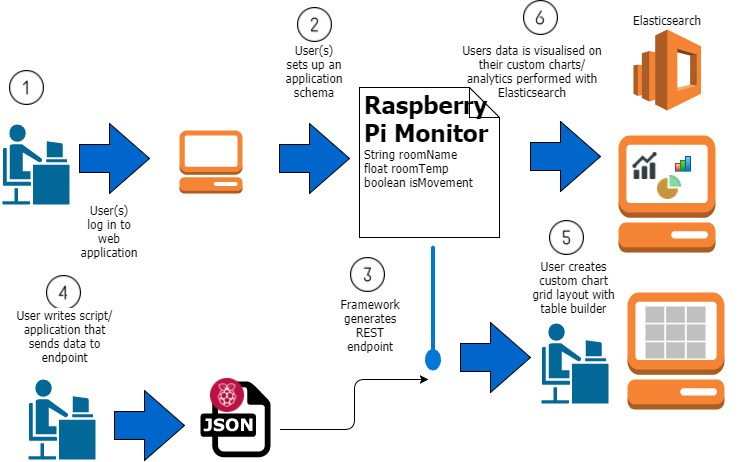
\includegraphics[width=\textwidth,height=\textheight,keepaspectratio]{dynamic_performance_framework_pi_flow}
In this example the user creates a schema in Iris for a raspberry pi. The user has a raspberry pi set up with a sensor to act as a home alarm. The user has written a script on the pi to send JSON data to the schema endpoint in Iris containing room name, room temperature and if there is any movement in the room. Data is being sent every five seconds to Iris. The user then logs into Iris and creates a dashboard for visualising the raspberry pi data.
\end{tcolorbox}
\caption{Raspberry Pi Monitor for Iris}
\end{figure}

\begin{figure}[H]
\begin{tcolorbox}
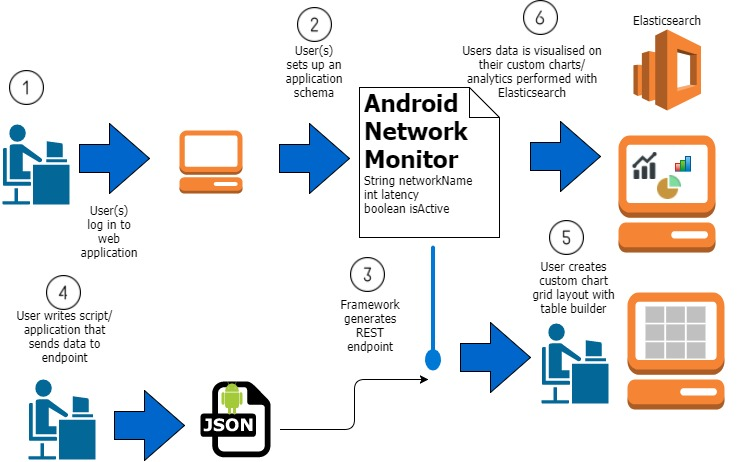
\includegraphics[width=\textwidth,height=\textheight,keepaspectratio]{dynamic_performance_framework_android_flow}
In this example the user creates a schema in Iris for an android application. The android application is sending network data to the Iris generated endpoint, the user sends the network name, latency and if the network is currently active in the form of a JSON object, every five seconds. The user then logs into Iris and build a dashboard to visualise the android data coming into Iris.
\end{tcolorbox}
\caption{Android Network Monitor for Iris}
\end{figure}

\chapter{Relevant Technologies}

In this chapter the technologies that will be used and the rationale for their selection, in the development of the Iris system are outlined. One section in particular Generating Dynamic Elasticsearch Queries is long but is important because the choice of technology is not obvious and the advantages/disadvantages of the alternatives is of particular importance to Onaware.

\section{Grails}

Iris will be built using the MVC web framework Grails. Grails is suited to for Iris due its rapid scaffolding capabilities, meaning a web application with CRUD (Create, Read, Update, Delete) actions can be implemented extremely fast. Due to the scale of the project a framework which will provide a fast POC (Proof of Concept) is needed, due to Grails’ command line interface a web application skeleton can be auto generated in a couple of commands. 

Also a significant factor in selecting Grails is that Onaware have several of their applications written using Grails and Iris will have a new lifecycle after this project cycle in which Onaware developers will be extending upon Iris. 

\section{Groovy}

Groovy is used by default within the Grails framework, this is a major factor as to why the technology is being used in Iris. However due to Grails being built on the JVM pure Java code could be used instead of Groovy, the major advantages of using Groovy over Java is its expressive nature and syntactic sugar, which allow you to write less code and do more. Groovy integrates seamlessly with any Java library, which is a major factor for using Groovy in Grails. Due to the popularity of Java, if Grails doesn’t have a native plugin for some needed functionality, a Java library more than likely exists to provide the required functionality, this library can then be used with Groovys expressive syntax.

\begin{figure}[H]
\begin{tcolorbox}
\begin{minted}{groovy}
//dynamic typing, will be cast as a string
def name = 'Dean'

//built in regex support
def matches = (name ==~ /\w+/)   

def message = (matches) ? "Matches" :
		 "No match found in string $name"

println message
\end{minted}
Output:
Matches
\end{tcolorbox}
\caption{Example of Groovy Syntax}
\end{figure}

\section{Spock}
Spock (\url{http://spockframework.org/spock/docs/1.1/getting_started.html}) is the default testing framework for Groovy and due to Grails using Groovy as its primary language. All unit and integration tests are written using the Spock framework. An advantage of the spock framework is that assertions are written in a behavior driven manner, which makes tests clear and concise unlike other JVM testing frameworks such as JUnit which relies on simple assertions.

\begin{figure}[H]
\begin{tcolorbox}
\begin{minted}{groovy}
void "test delete Schema"(){
	setup:
	setupData()

	when: "I delete a Schema"
	schema.delete(flush: true)

	then: "It is deleted from the database"
	assert Schema.count() == 0
}
\end{minted}
\end{tcolorbox}
\caption{Example of Spock Test in Iris}
\end{figure}
Peter Niederwieser has a concise introduction tutorial on Spock at the following link \url{ http://spockframework.org/spock/docs/1.1/introduction.html }

\section{Elasticsearch}

Elasticsearch is a RESTful based search engine for indexing documents of data. Elasticsearch is suited for Iris as it accepts structured data in the form of index mappings, as well as unstructured data. 

\begin{figure}[H]
\begin{tcolorbox}
PUT twitter
\begin{minted}{json}
{
   "mappings":{
      "tweet":{
         "properties":{
            "message":{
               "type":"text"
            }
         }
      }
   }
}
\end{minted}
An example of an Elasticsearch mapping being set up for an index - \url{ https://www.elastic.co/guide/en/elasticsearch/reference/current/indices-put-mapping.html}
\end{tcolorbox}
\caption{Example of an Elasticsearch Mapping}
\end{figure}

There are alternatives to Elasticsearch, in particular  Hadoop and Spark. However, the main reason for using Elasticsearch is that Onaware developers have experience using Elasticsearch on their other products, so to maintain the product after the project lifecycle Elasticsearch is the best choice for Onaware as they can remain consistent with their technologies.

Another reason for Elasticsearch being used in Iris was due it being RESTful. All data coming to Iris will be made with REST calls already in the correct format for Elasticsearch, meaning a simple redirect to an Elasticsearch URL allows Iris to insert a user’s data to Elasticsearch. Querying Elasticsearch is also a major part of Iris and it can be done through REST calls using aggregations. Aggregations will allow Iris to come with out of the box analytics that can be easily mapped to a user's chart. As aggregations are the backbone of Iris an aggregation playground will be put in place where a user can build up complex aggregations using a user friendly interface and send them to Elasticsearch. 

\subsection{Generating Dynamic Elasticsearch Queries}
\subsubsection{Elasticsearch Java API Issue}
Elasticsearch comes with a rich Java API for using Elasticsearch in your applications. The API covers all features of Elasticsearch which Iris requires such as creating indices, mapping indices and performing and parsing aggregations. The main issue with the Java API is that it doesn’t expand well in Iris due to Iris dealing with dynamic data. The Java API is set up in a such a way that if a user wishes to create a complex aggregation with several sub-aggregations Iris would have to  use reflection or have several complex factory design patterns in place. This approach is not ideal, and is best explained with an example using the Java API:
\begin{figure}[H]
\begin{tcolorbox}
POST /exams/\_search?size=0
\begin{minted}{json}
{
   "aggs":{
      "avg_grade":{ "avg":{"field": "grade"}}
   }
}
\end{minted}
An example of an average aggregation being performed on a field ‘grade’. As you can see an aggregation is just a JSON object which works upon a given field.
However when you use the Java API building a similar aggregation without knowing beforehand what the data looks like would be quite difficult and may require reflection in the language you are using. Below is an example of a simple aggregation with a sub aggregation being created using the Java API. \url{https://www.elastic.co/guide/en/elasticsearch/reference/current/search-aggregations-metrics-avg-aggregation.html}

\begin{minted}{java}
AggregationBuilders
	.terms("genders")
	.fields("gender")
	.order(Terms.Order.aggregation("avg_height", false)
	.subAggregation(
	   AggregationBuilders.avg("avg_height")
			              .field("height")
	)
\end{minted}
Looking at this example of the Java API, the first method call to ‘terms’, references an aggregation type and the next call adds the ‘gender’ field to the aggregation. An Optional order is added to the aggregation, notice how a static call to ‘Terms.Order.aggregation’ is used. Finally a sub aggregation is added, which refers to the average aggregation. From the example notice the large amount of calls to static methods, this would require Iris to have a factory in place for each aggregation type, which is possible. The problem occurs when users wish to add extra attributes such as ordering to an aggregation, as Iris would need a factory in place for every possible form of an aggregation. Once again this is possible, but not a very elegant way of building up a JSON object, as a user may not wish to use all of the available optional attributes.
\end{tcolorbox}
\caption{Example Aggregation for Elasticsearch}
\end{figure}
The API is catered more towards having prebuilt aggregations in the backend where you can just fill in the blank parts of the aggregation with fields and is not the best for building aggregations from scratch due to the amount of code needed to fit with the existing API. It is for this reason Iris will implement its own approach for building aggregations.

\subsubsection{Solution using Groovy/Grails}
Groovy is an excellent candidate as Groovy objects are essentially just maps of keys and values which can be converted into JSON using standard Groovy functions. Groovy constructors will only use the fields given to it and add default values to the remaining fields which were not specified. With this knowledge Elasticsearch aggregation objects built in Groovy would automatically support optional attributes such as order, sort etc… 
\begin{figure}[H]
\begin{tcolorbox}
\begin{minted}{groovy}
import Groovy.json.JsonBuilder 

class Person{     
    String name 
    int age
}  

// age will be given a default value
def person1 = new Person(name: 'dean') 

 //notice the key/value style constructor
def person2 = new Person(name: 'shane', age: 20) 

Map personMap = [name: 'kieran', age: 30]
//object constructed from a map
def person3 = new Person(personMap)

println new JsonBuilder(person1).toPrettyString()
println new JsonBuilder(person2).toPrettyString()
println new JsonBuilder(person3).toPrettyString()​
\end{minted}
Output:
\begin{minted}{json}
{
    "age": 0,
    "name": "dean"
}
{
    "age": 20,
    "name": "shane"
}
{
    "age": 30,
    "name": "kieran"
}
\end{minted}
\end{tcolorbox}
\caption{Example of Groovy Constructor}
\end{figure}
\pagebreak
The Groovy implementation follows a standard OOP (Object Orientated Programming) approach. Each Aggregation type is given a class with optional fields, similar to the example above, a factory then accepts a map coming from the front end along with the name of the aggregation type and creates the correct object using the map.
\begin{figure}[H]
\begin{tcolorbox}
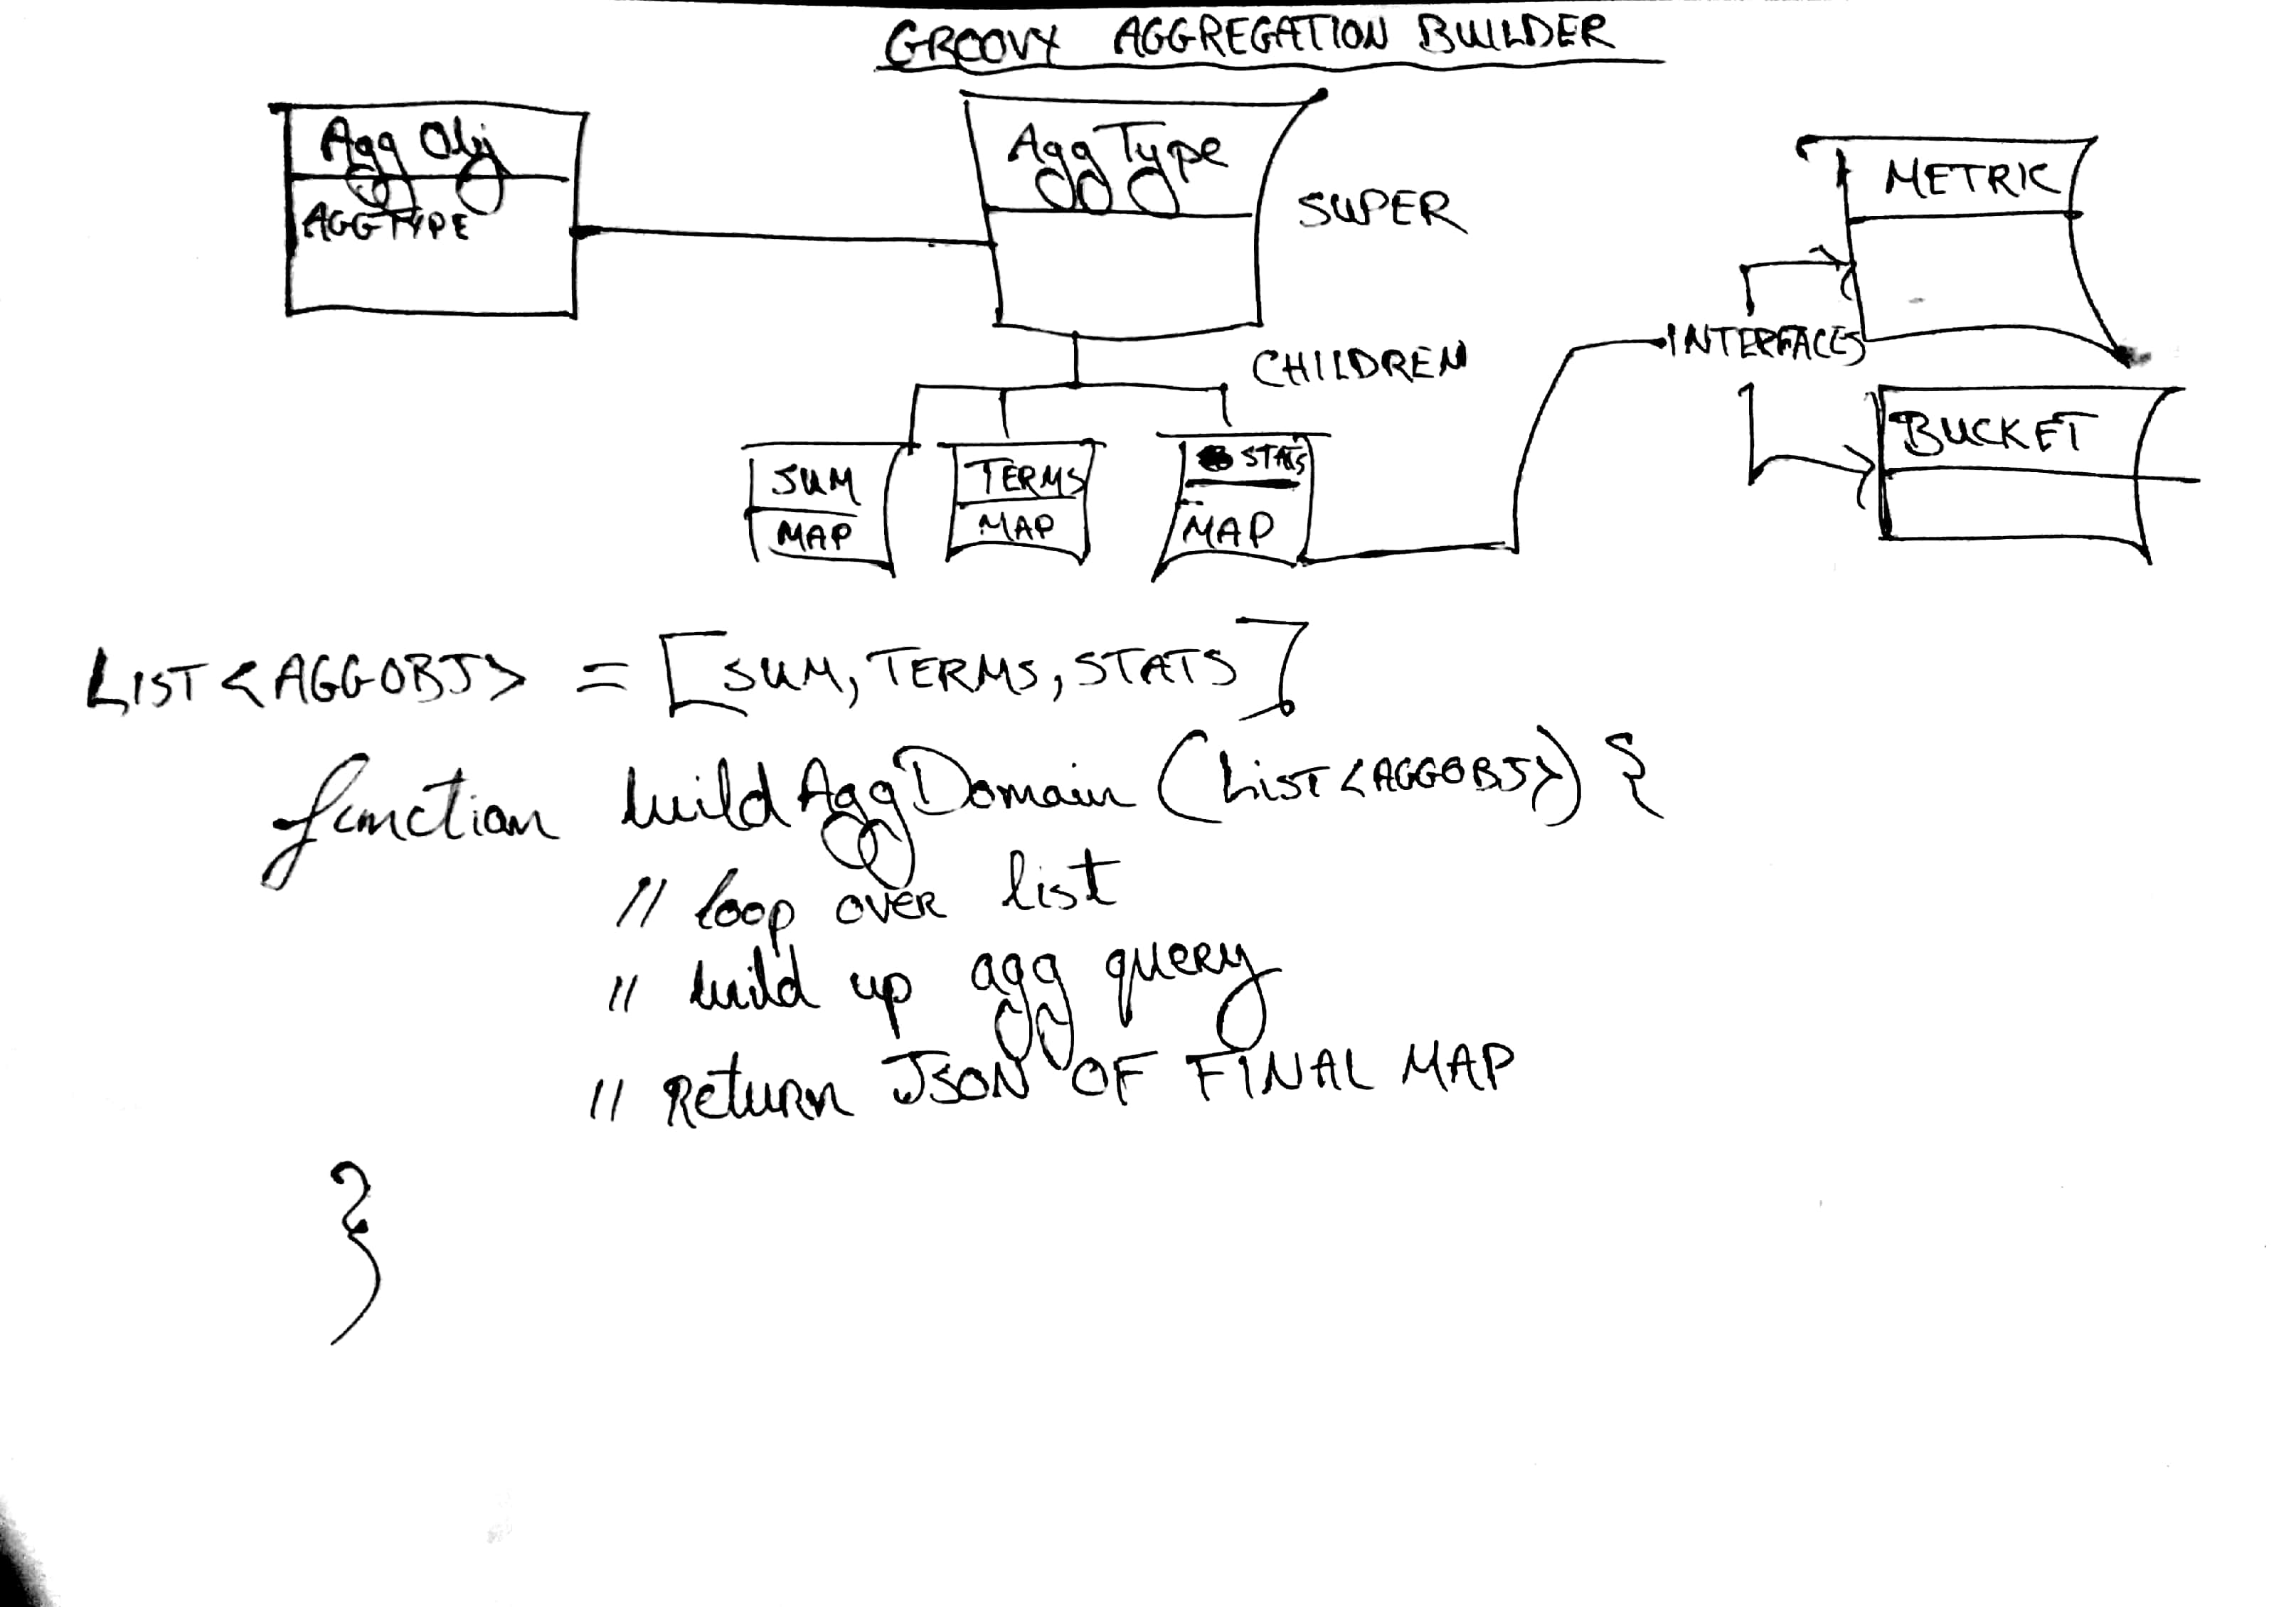
\includegraphics[width=\textwidth,height=\textheight,keepaspectratio]{groovy_agg_builder_logic_1}
This diagram shows how a Groovy implementation of Elasticsearch aggregations may look and how they may be built into a single object.
\end{tcolorbox}
\caption{Iris Aggregation Implementation POC}
\end{figure}
\begin{figure}[H]
\begin{tcolorbox}
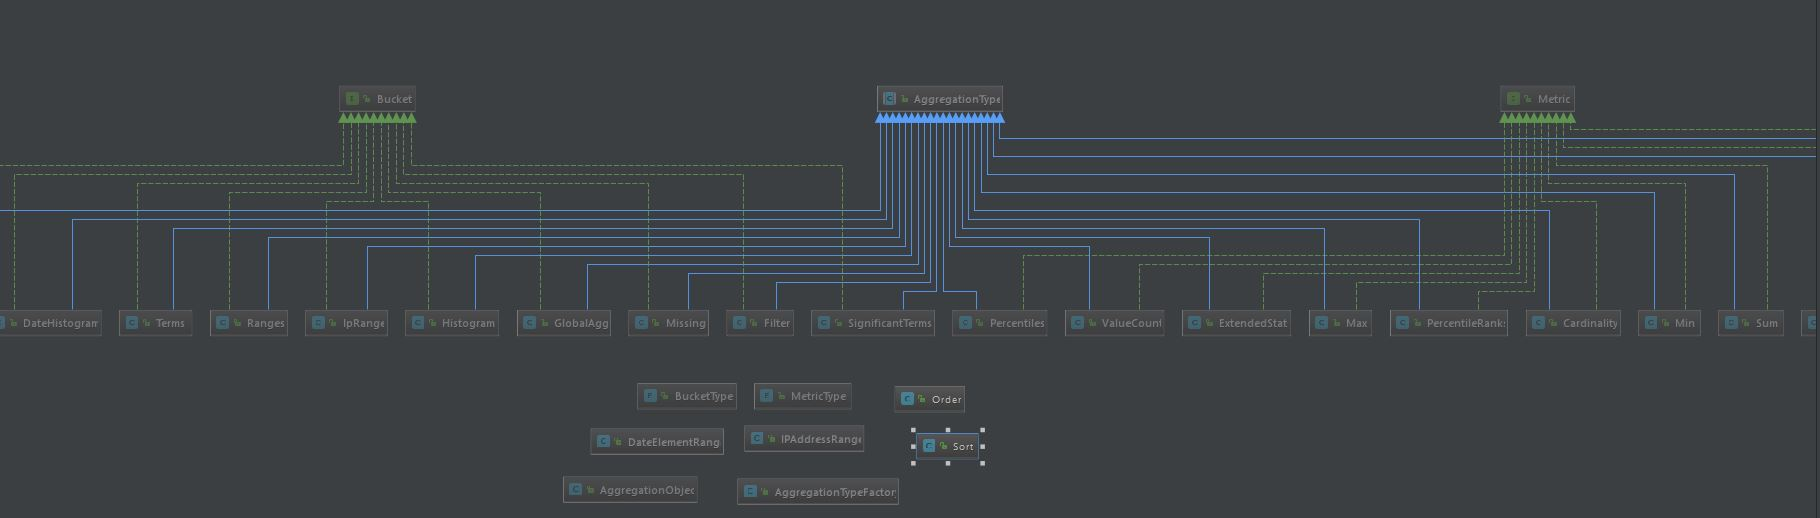
\includegraphics[width=\textwidth,height=\textheight,keepaspectratio]{intellij_agg_diagram}
The diagram\footnotemark above is a screenshot from IntelliJ. The diagram shows my Groovy implementation class structure.
\end{tcolorbox}
\caption{Iris Aggregation Groovy Implementation}
\end{figure}
\footnotetext{This figure is for illustrative purposes only, to demonstrate the level of complexity required in the Groovy implementation.}
\paragraph{Advantages of using Groovy/Grails}
\begin{itemize}
  \item Groovy constructors are maps which can assign default values
  \item OOP approach
  \item Scalable, can be updated easily to match Elasticsearch aggregations
  \item Addition and removal of aggregation classes without system interference
\end{itemize}
\paragraph{Disadvantages of using Groovy/Grails}
\begin{itemize}
  \item Link between frontend and backend requires complex command objects
  \item Command objects become very hard to maintain, as it must be index within HTML
\end{itemize}
An example of how command objects work can be found here:
\newline
\url{http://guides.grails.org/command-objects-and-forms/guide/index.html}
\subsubsection{Solution using Javascript}
Currently a separate implementation is in development for Iris to deal with aggregation objects using Javascript. This implementation depends on building the aggregation object dynamically from user input on the front end. As the user builds the aggregation object on the front end, an aggregation JSON object is being built along with it, this JSON object will then be saved in Iris as a String object.
\begin{figure}[H]
\begin{tcolorbox}
\centerline{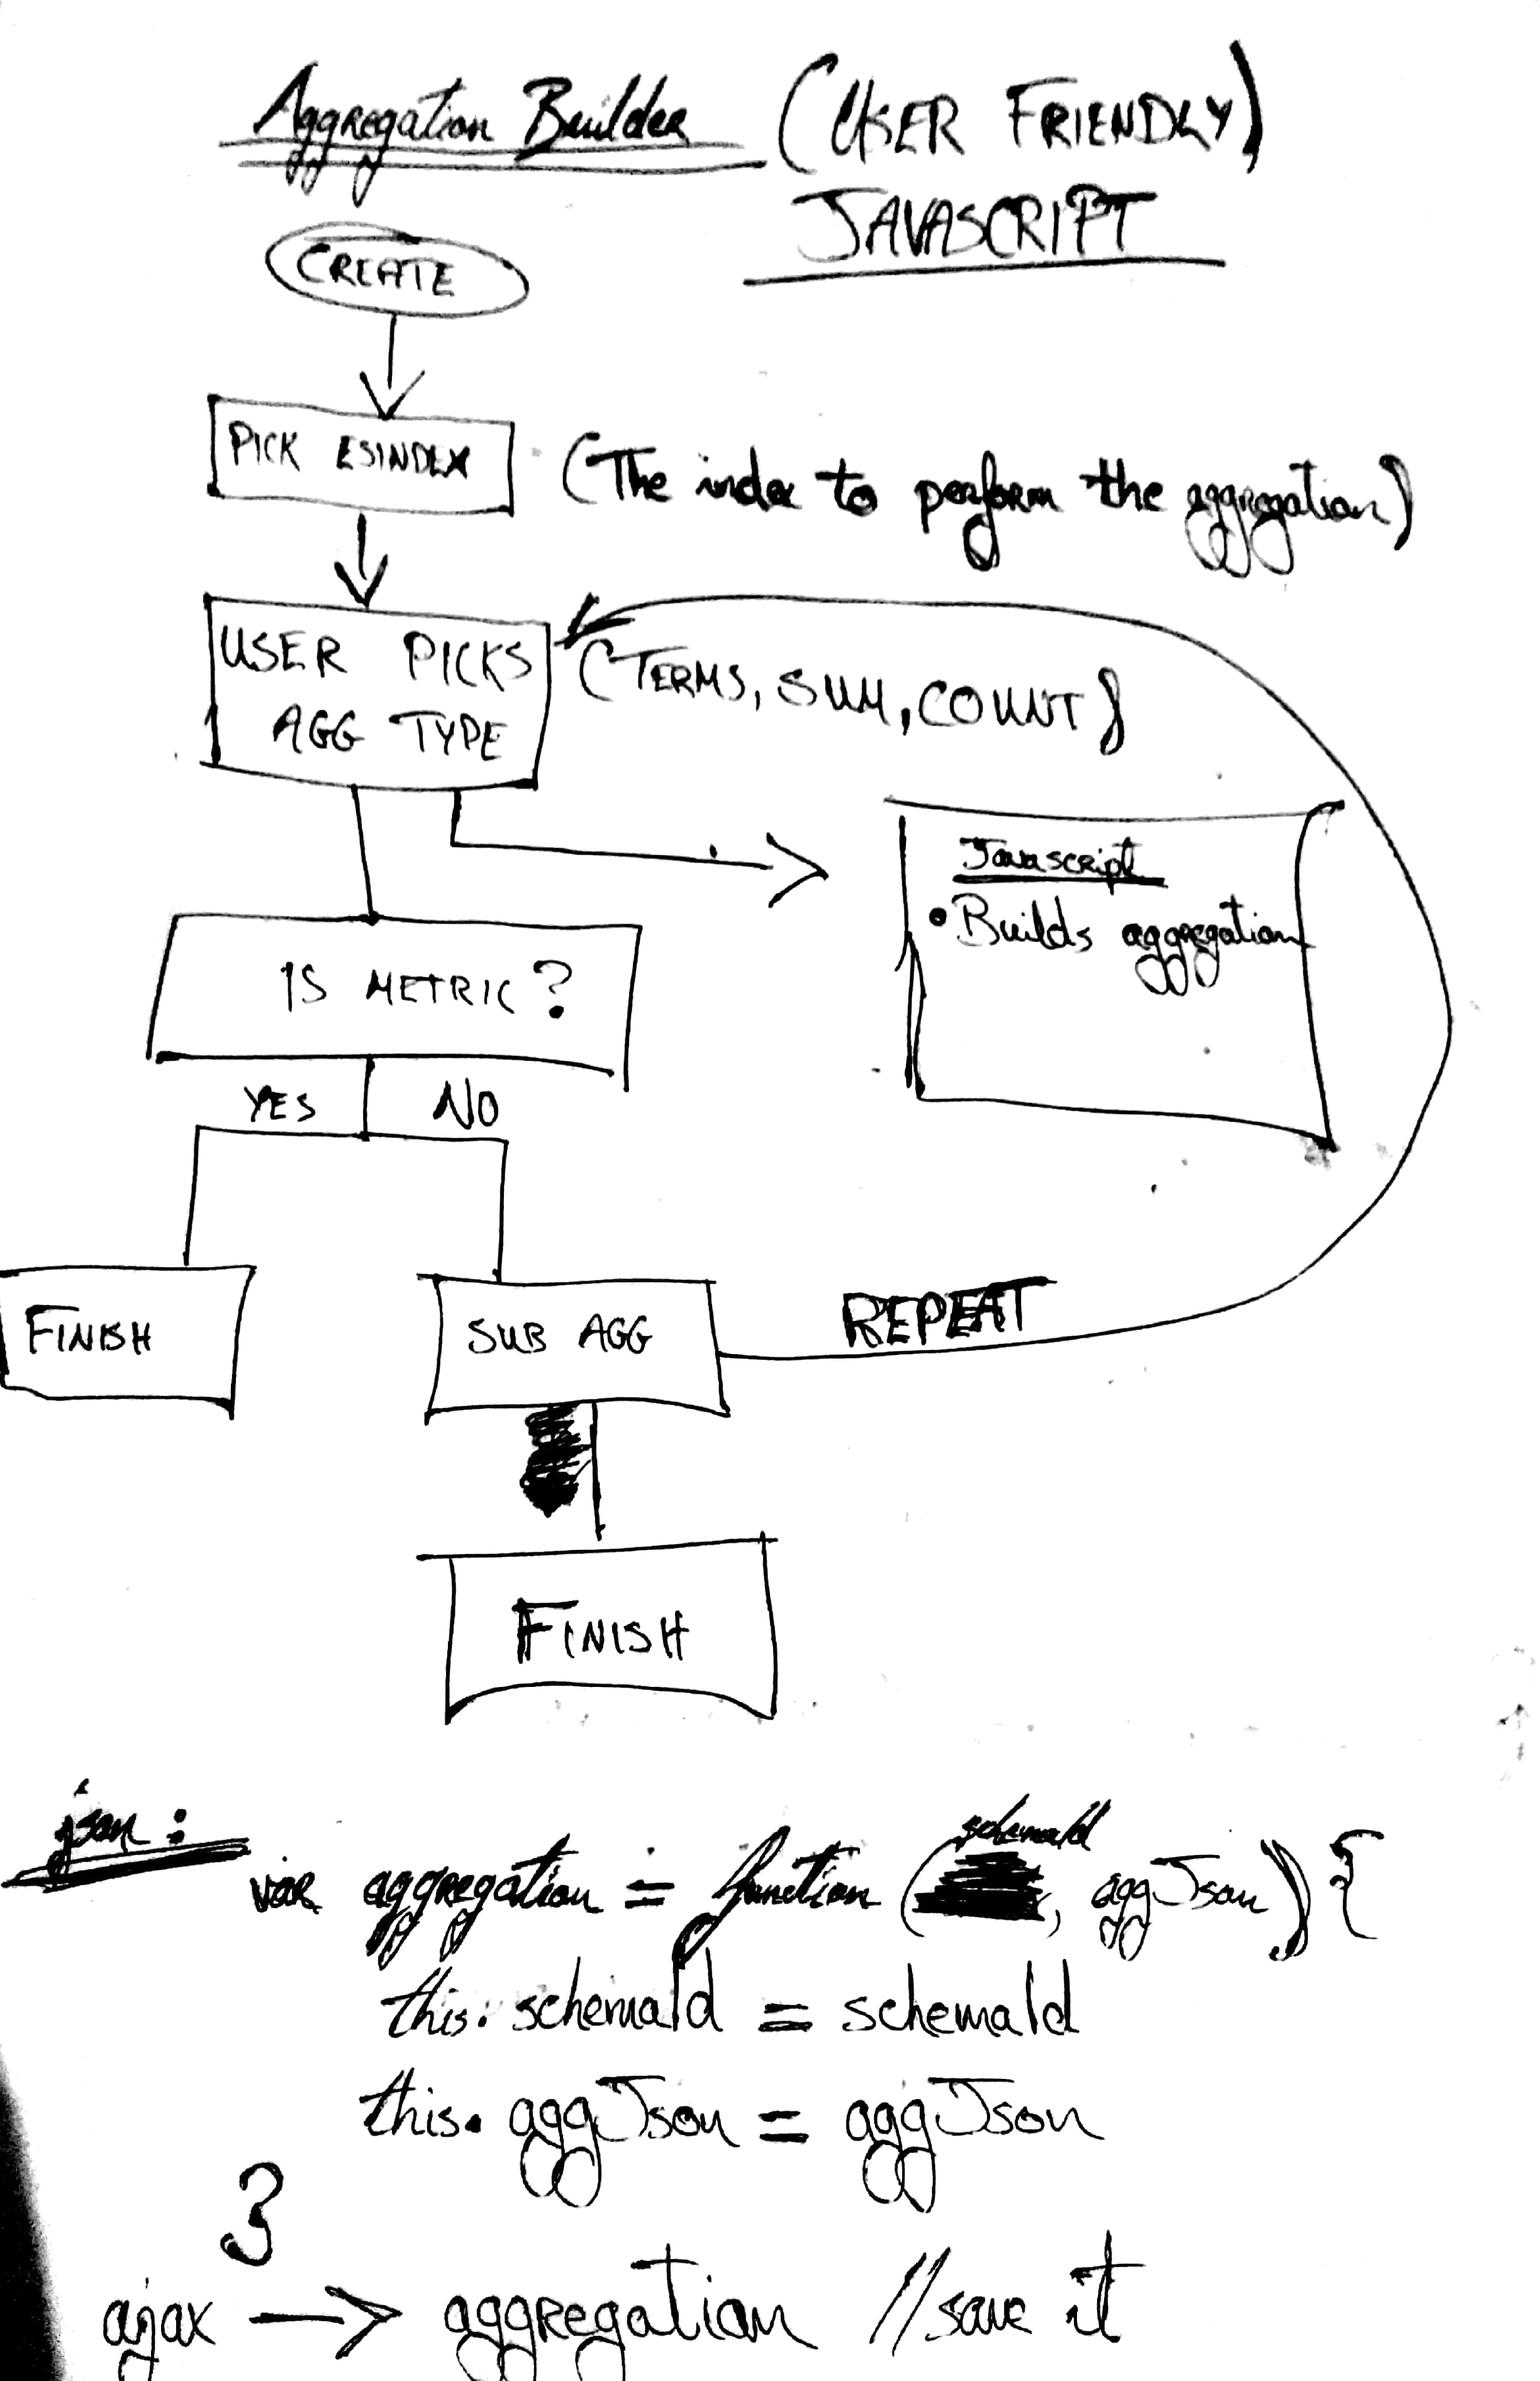
\includegraphics[width=\textwidth]{js_agg_builder_flow_1}}

This diagram shows the flow of how a user would create an aggregation using the frontend of Iris and shows how the Javascript builds the aggregation incrementally.
\end{tcolorbox}
\caption{Javascript Implementation POC}
\end{figure}

\paragraph{Advantages of using Javascript}
\begin{itemize}
\item Keep the aggregation object in its native language, JSON
\item Remove 15 - 20 Groovy classes with a single Javascript file
\item Store JSON as a string in database, making it immediately executable
\item Balances load on the server, as clients now build aggregations
\end{itemize}
A practical tutorial on Elasticsearch aggregations and sub-aggregations can be found here \url{https://qbox.io/blog/elasticsearch-aggregations-for-analytics}

\section{JQuery}
JQuery (\url{http://api.jquery.com}) will be used to post form data, make ajax calls as well as traversing and manipulating the DOM (Document Object Model). JQuery is a defacto industry standard library for accomplishing these tasks.

\section{Grails Spring Websockets Plugin}
This plugin will be used mainly for updating charts. The sockets will allow for charts to be updated as soon as new data comes into Iris. The Spring plugin allows a Grails Service or Controller to deal with passing data to specific endpoints. These endpoints are referred to as STOMP (Simple [or Streaming] Text Orientated Messaging Protocol) endpoints (Docs.spring.io, 2017). It is then possible for Iris to target charts specific to a schema, which is much more efficient than all charts receiving all data. Controlling STOMP endpoints in Iris can be taken a step further by creating dynamic STOMP endpoints which would be specific to both a schema a chart type, meaning a pie chart could subscribe to an endpoint only related to pie charts, so the data being sent to the pie chart subscriber will already be formatted for pie charts. This once again prevents charts receiving data which is not relevant to them. The endpoints are secured with the Spring Security plugin.
\begin{figure}[H]
\begin{tcolorbox}
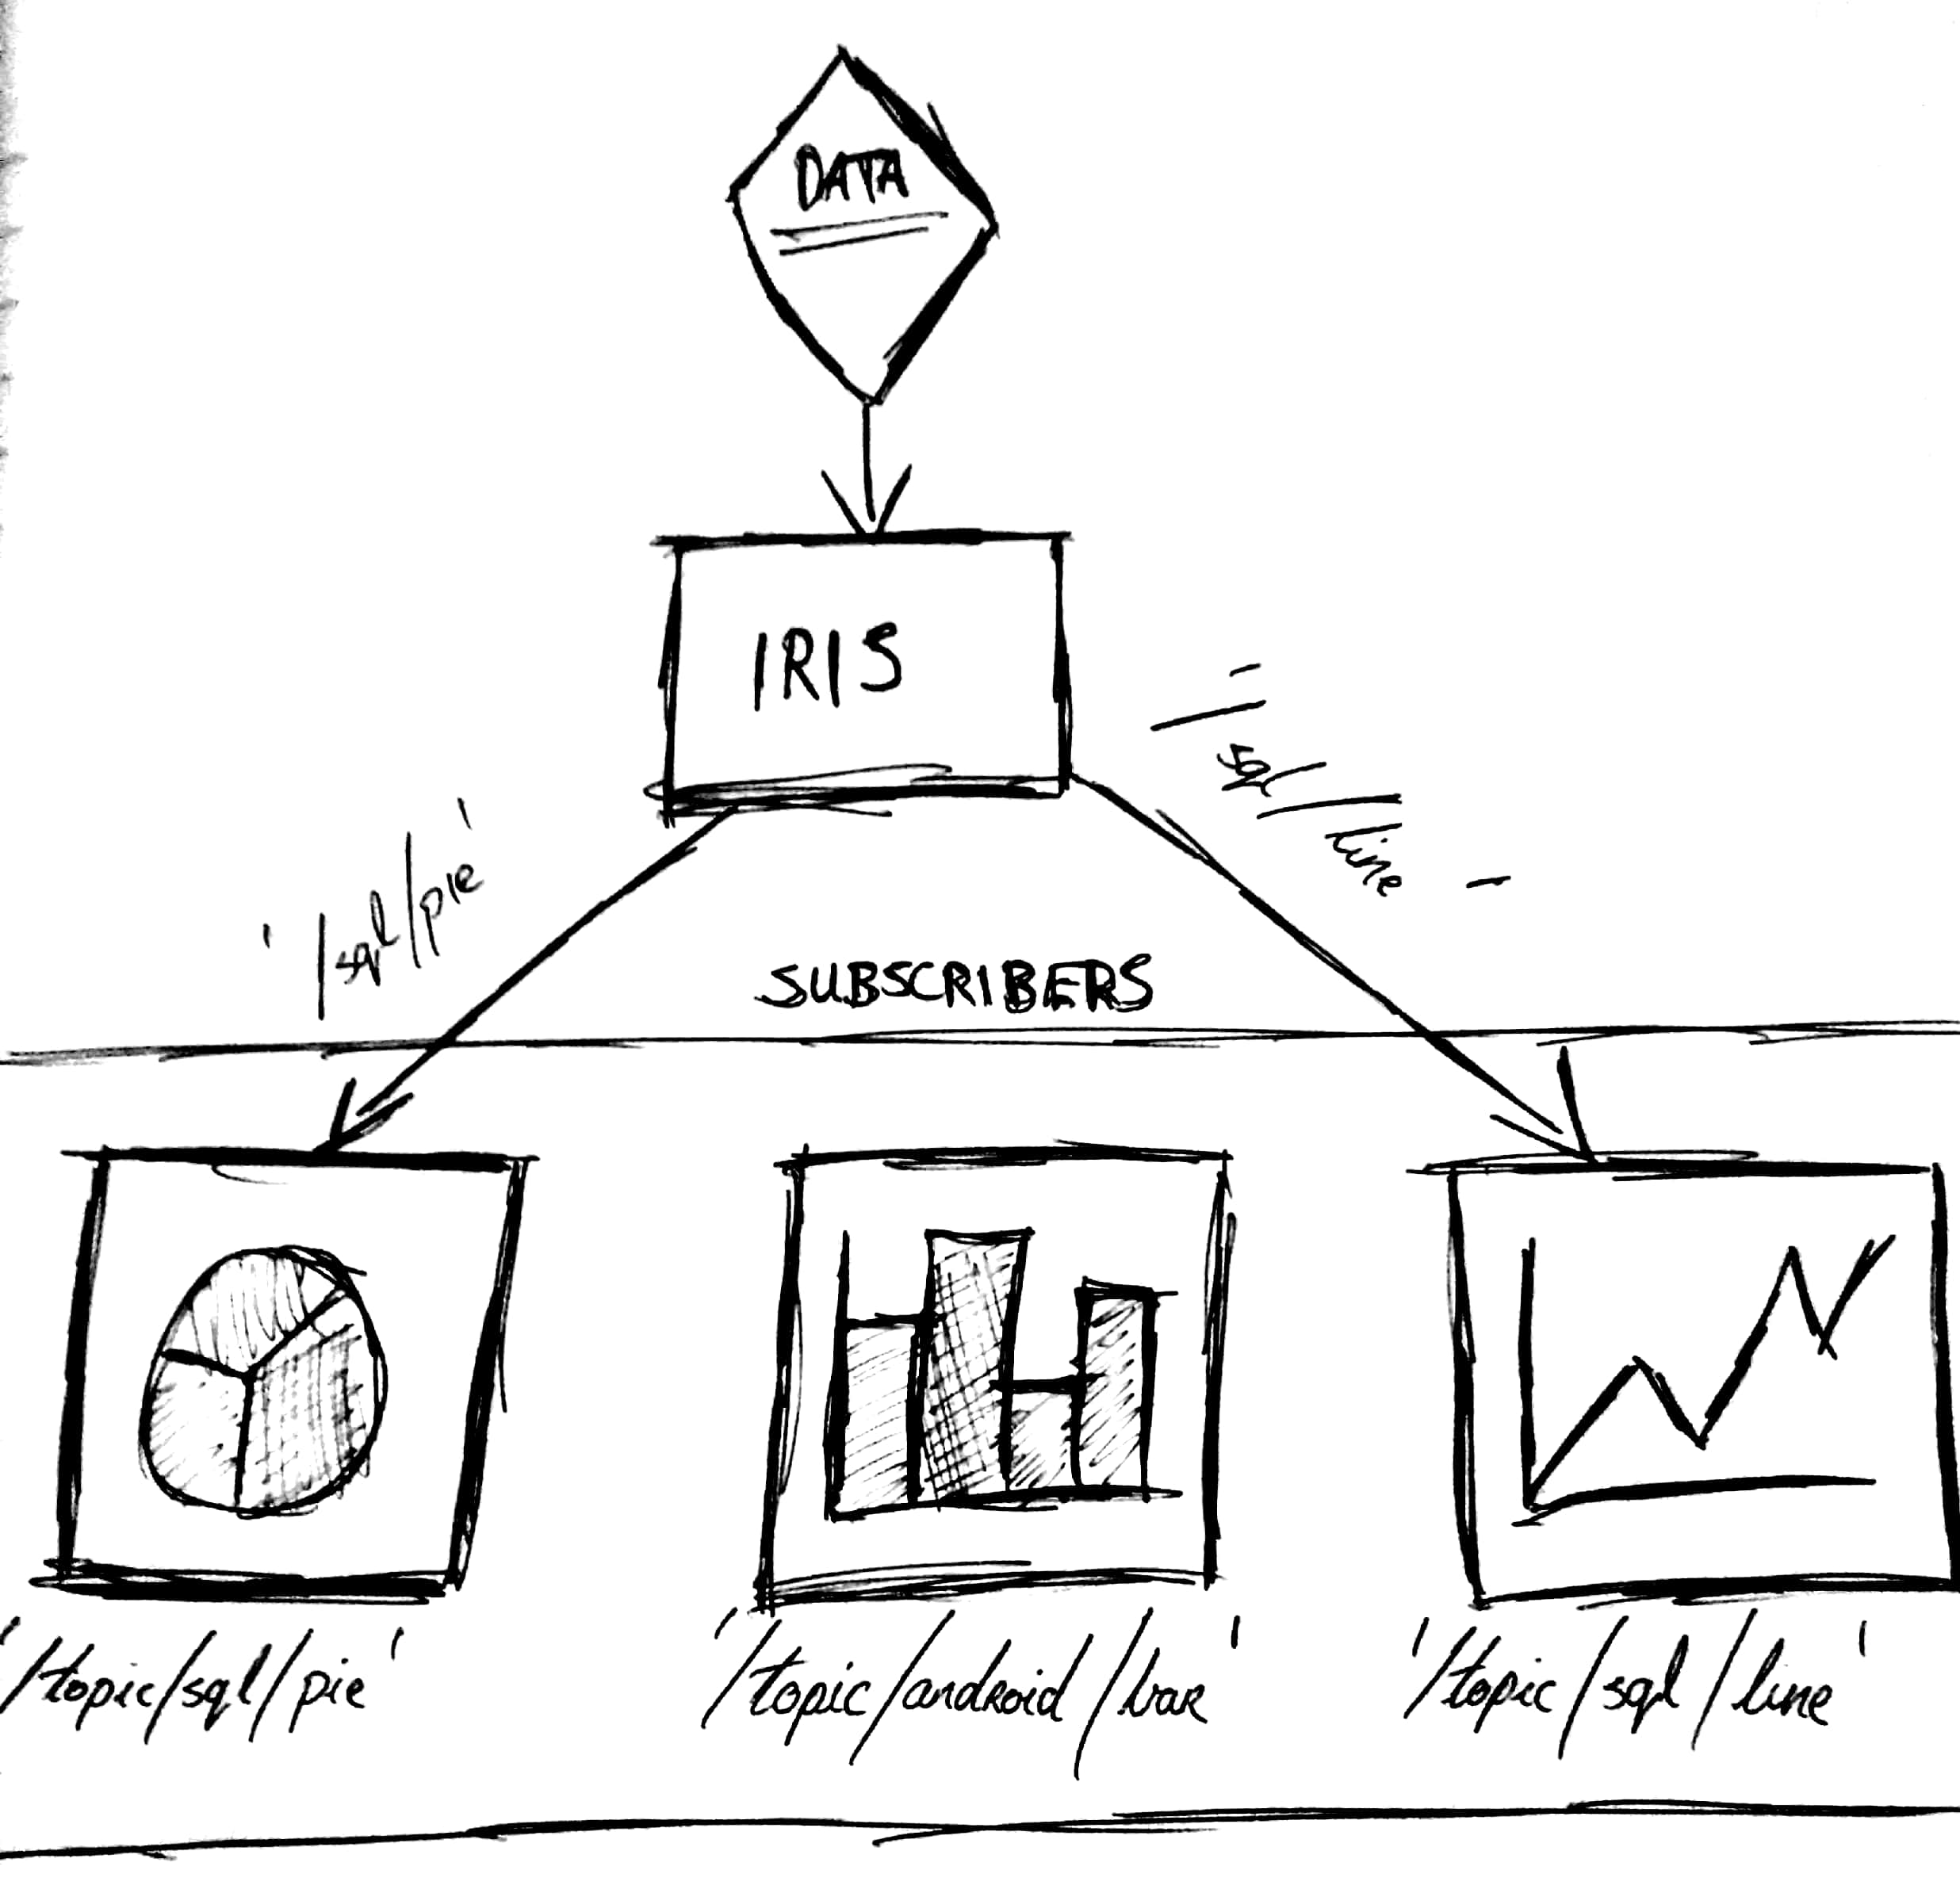
\includegraphics[width=\textwidth,height=\textheight,keepaspectratio]{iris_sockets}
\newline
The diagram above shows data coming into Iris. The data coming into Iris is for a schema called ‘sql’. Iris sends out data to \q{/sql/pie} and \q{/sql/line}, this means any pie charts or line charts associated with the \q{sql} schema will receive the data and be updated. This is shown by the pie chart and line chart subscribing to the correct topics \q{/topic/sql/pie} and \q{/topic/sql/line}. The bar chart is subscribed to an endpoint called \q{/topic/android/bar} which will not receive any updates as no data has been sent to Iris related to the \q{android} schema.
\end{tcolorbox}
\caption{Iris Socket POC}
\end{figure}
For documentation on the Grails Spring Websockets plugin see \url{https://plugins.grails.org/plugin/zyro/grails-spring-websocket}

\section{Selenide (Functional Testing)}
Selenide (\url{http://selenide.org/documentation.html}) will be used for functional tests in Iris. Selenide is a wrapper library for Selenium which removes the boilerplate code for Selenium such as Implicit and Explicit waits. Selenide allows your tests to be more clear and concise due to its expressive function naming convention. Selenide also uses Javascript style selectors to make the developer feel as though they are targeting DOM elements using Javascript rather than Java.

\section{Dashboards}

Iris will allow users to create dashboards which consist of charts, the dashboard tiles should be moveable and resizable and most importantly serializable.
\subsection{ Dashboard Library Requirements}
\begin{itemize}
\item Moveable tiles
\item Resizeable tiles
\item Adding tiles
\item Removing tiles
\item Have serializable functionality
\item Be under an MIT License so Onaware may use it
\item Active Developer Support (Optional, but preferable)
\end{itemize}

\subsection{Review of Dashboard Libraries}

Four libraries were researched in the design process of Iris’ dashboard system. Refer to Appendix~\ref{sec:dashboards} for a detailed comparison of the dashboard libraries. Below is a table summarising the comparisons.
\begin{table}[H]
\centering
\small
\setlength\tabcolsep{2pt}
 \begin{tabular}{|c|c|c|c|c|c|c|c|c|}
 \hline
 	& Moveable & Resizable & Add Tiles & Remove &  & MIT & Active\\[-3pt]
Library & Tiles &   Tiles &   Dynamically &   Tiles & Serializable  &   Licensed &  Support\\
 \hline\hline
 Gridster & \checkmark & \checkmark & \checkmark &\checkmark & \checkmark & \checkmark & \xmark\\ 
 \hline
 Packery & \checkmark & \checkmark & \checkmark &\checkmark & \xmark & \xmark & \xmark\\ 
 \hline
 GridList & \checkmark & \checkmark & \xmark &\xmark & \checkmark & \checkmark & \xmark\\ 
 \hline
 Gridstack & \checkmark & \checkmark & \checkmark &\checkmark & \checkmark & \checkmark & \checkmark\\ 
 \hline
\end{tabular}
\caption{Dashboard Review}
\end{table}

\section{Chart Libraries}
\subsection{Chart Library Requirements}
\begin{itemize}
\item D3v4 wrapper library or better alternative to D3
\item Support basic chart types (Bar, Bubble, Pie, Line, \ldots)
\item Out of the box legends, zooming and responsiveness
\item Allow for chart updates without the need for redrawing
\item JSON data support
\item Active Developer Support (Optional, but preferable)
\item Advanced Chart Types (Radar, Heatmap, \ldots)
\end{itemize}

\subsection{Review of Chart Libraries}
Four libraries were researched in the design process of Iris’ charting system. 
Refer to Appendix~\ref{sec:charts} for a detailed comparison of the chart libraries as well as a information on why D3 is not being used for Iris. Below is a table summarising the comparisons.

\begin{table}[H]
\centering
\small
\setlength\tabcolsep{2pt}
 \begin{tabular}{|c|c|c|c|c|c|c|c|c|}
 \hline
  	      & D3v4 - 	&  Basic    & Advanced &Included & Updateable & JSON & Active\\[-3pt]
  Library  &   Wrapper &  Charts & Charts & Functionality & Charts & Support & Support\\
 \hline\hline
 C3 & \xmark & \checkmark & \checkmark &\checkmark & \checkmark & \checkmark & \xmark\\ 
 \hline
 Billboardjs & \checkmark & \checkmark & \checkmark &\checkmark & \checkmark & \checkmark & \checkmark\\ 
\hline
 Chartjs & \checkmark & \checkmark & \xmark & \checkmark & \checkmark & \checkmark & \checkmark\\ 
 \hline
\end{tabular}
\caption{Chart Libary Review}
\end{table}

\section{Similar Products}
\subsection{Kibana}

Kibana (\url{https://www.elastic.co/guide/en/kibana/5.6/getting-started.html}) is a web application which allows you to visualise your ELK (Elasticsearch, Logstash, Kibana) stack. Kibana supports aggregations to be performed on Elasticsearch data and the visualisation of aggregations using charts and metrics. Kibana also supports persistent dashboards, however they are not personal dashboards meaning all users with access to the Kibana instance can view and modify the same dashboards, which is an unusual design choice (Logz.io, 2017). Kibana does not have any concept of a user, meaning there are no personal aspects to the application. Kibana also doesn’t have any user friendly ways to insert data into Elasticsearch meaning you have to understand Elasticsearch concepts in order to use Kibana. Kibana is also aimed towards managing and visualising log data rather than generic data. 

\subsection{Grafana}

Grafana (\url{http://docs.grafana.org/features/datasources/elasticsearch/}) is an open source dashboard tool for visualising time series data. Grafana supports several backend data sources, including Elasticsearch. Each data source has a corresponding query editor for users to query their data. Grafana is extremely powerful and has a very active community where users can collaborate and share dashboards. Grafana has the same issues as Kibana and doesn’t allow a user to enter data into the data source without having background knowledge of the data source.

\subsection{New Relic}

New Relic (\url{https://newrelic.com/application-monitoring/features}) is a monitoring application which comes close to what Iris wishes to achieve. New Relic is mainly used for anticipating bottlenecks and issues with applications. It is extremely powerful and supports multiple languages (Java, Nodejs and Python) and frameworks however it won’t support data for unsupported languages and frameworks and is not dynamic — this is a fundamental feature of Iris.

\subsection{AWS (Amazon Web Services)}

AWS will be used for hosting an Elasticsearch instance which Iris can use throughout its development cycle. The advantage of using AWS is that Iris can query the Elasticsearch instance from any location making the development flexible.

\chapter{Iris Current Progress}

\section{Design Iterations}

Iris has had four design iterations up to this point. This section will talk about Iris’ current design. See Appendix~\ref{sec:iterations}, for details on the other design iterations of Iris. 

Iris’ development process is being carried out using the agile methodology of BDD (Behavior Driven Development). Iris is developed in iterations of two week sprints. Every two weeks Iris is branched over to a new branch and Trello is updated with a new label which corresponds to the branch number. Iris is currently on version 0.0.3. For more information on Trellos roll in the development of Iris please refer to Appendix B.

\subsection{Iris (Current)}

Fugure~\ref{fig:iris_uml} is a high level UML representation of the current implementation of Iris. 
This has been fully implemented and tested in Grails. Iris currently allows a user to create a schema with schema fields, which in turn creates Elasticsearch mappings and indices specific to the created schema. With a mapping setup Iris allows a user to target an endpoint to send their data, the logic for putting this data into Elasticsearch has been written and tested but it is not linked up yet.

\begin{figure}[h]
\begin{tcolorbox}
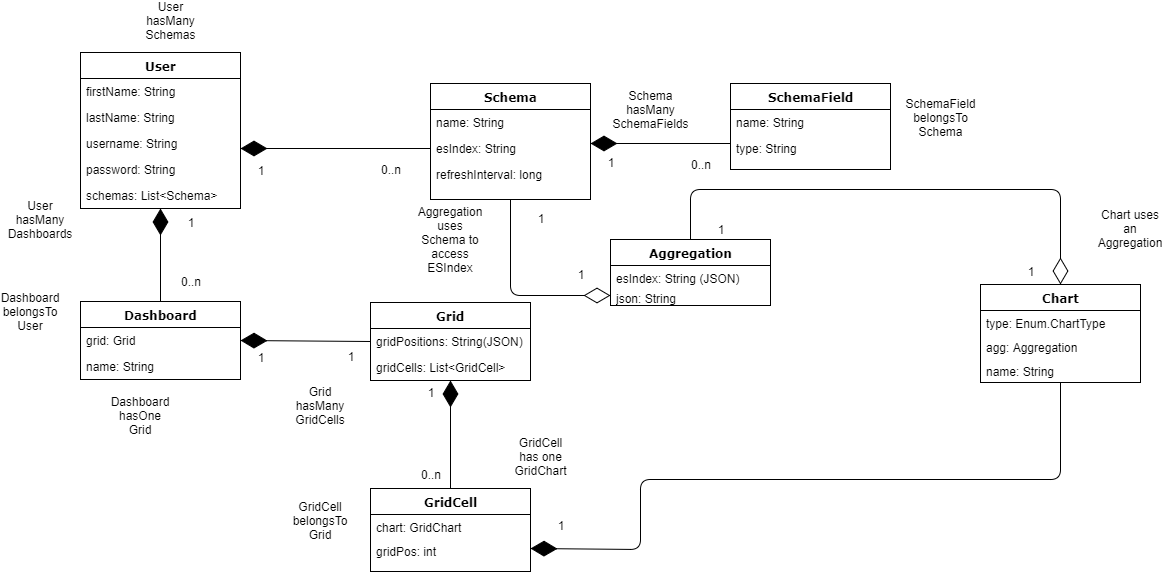
\includegraphics[width=\textwidth]{iris_models}
\end{tcolorbox}
\caption{Iris UML Diagram}\label{fig:iris_uml}
\end{figure}


Iris has an Elasticsearch instance hosted on AWS (Amazon Web Services) which will be used for the remainder of the development process.

Iris also has the two implementations of the aggregation building system in development. The Groovy version is completed but not linked to the backend, as progress on the Javascript version has begun which seems to be a more promising. It is likely that the Javascript version will completely replace the Groovy version. There is currently a single page application within Iris which allows a user to build up an aggregation on the front end which was completed using Javascript. This is still quiet rough on the front end, but proves that the Javascript logic works.

Iris also has a single hard coded chart which sits inside a gridstack grid (dashboard). The chart is being updated with randomly generated data being every five seconds to update the chart. This is to make sure data can be flushed smoothly to Billboardjs and ensure that the chart will not overflow inside of the dashboard grid.

As of now the next steps in the current sprint is to populate Elasticsearch with some real data and to develop the socket logic to allow charts to be updated when data is being routed to Iris. Serialization of dashboards is another time consuming task which must be implemented, but still needs to be planned out some more in order to ensure it is done properly. The front of end Iris is still rough, and the following diagram shows how the front end plans to interact with the backend.

\begin{figure}[H]
\begin{tcolorbox}
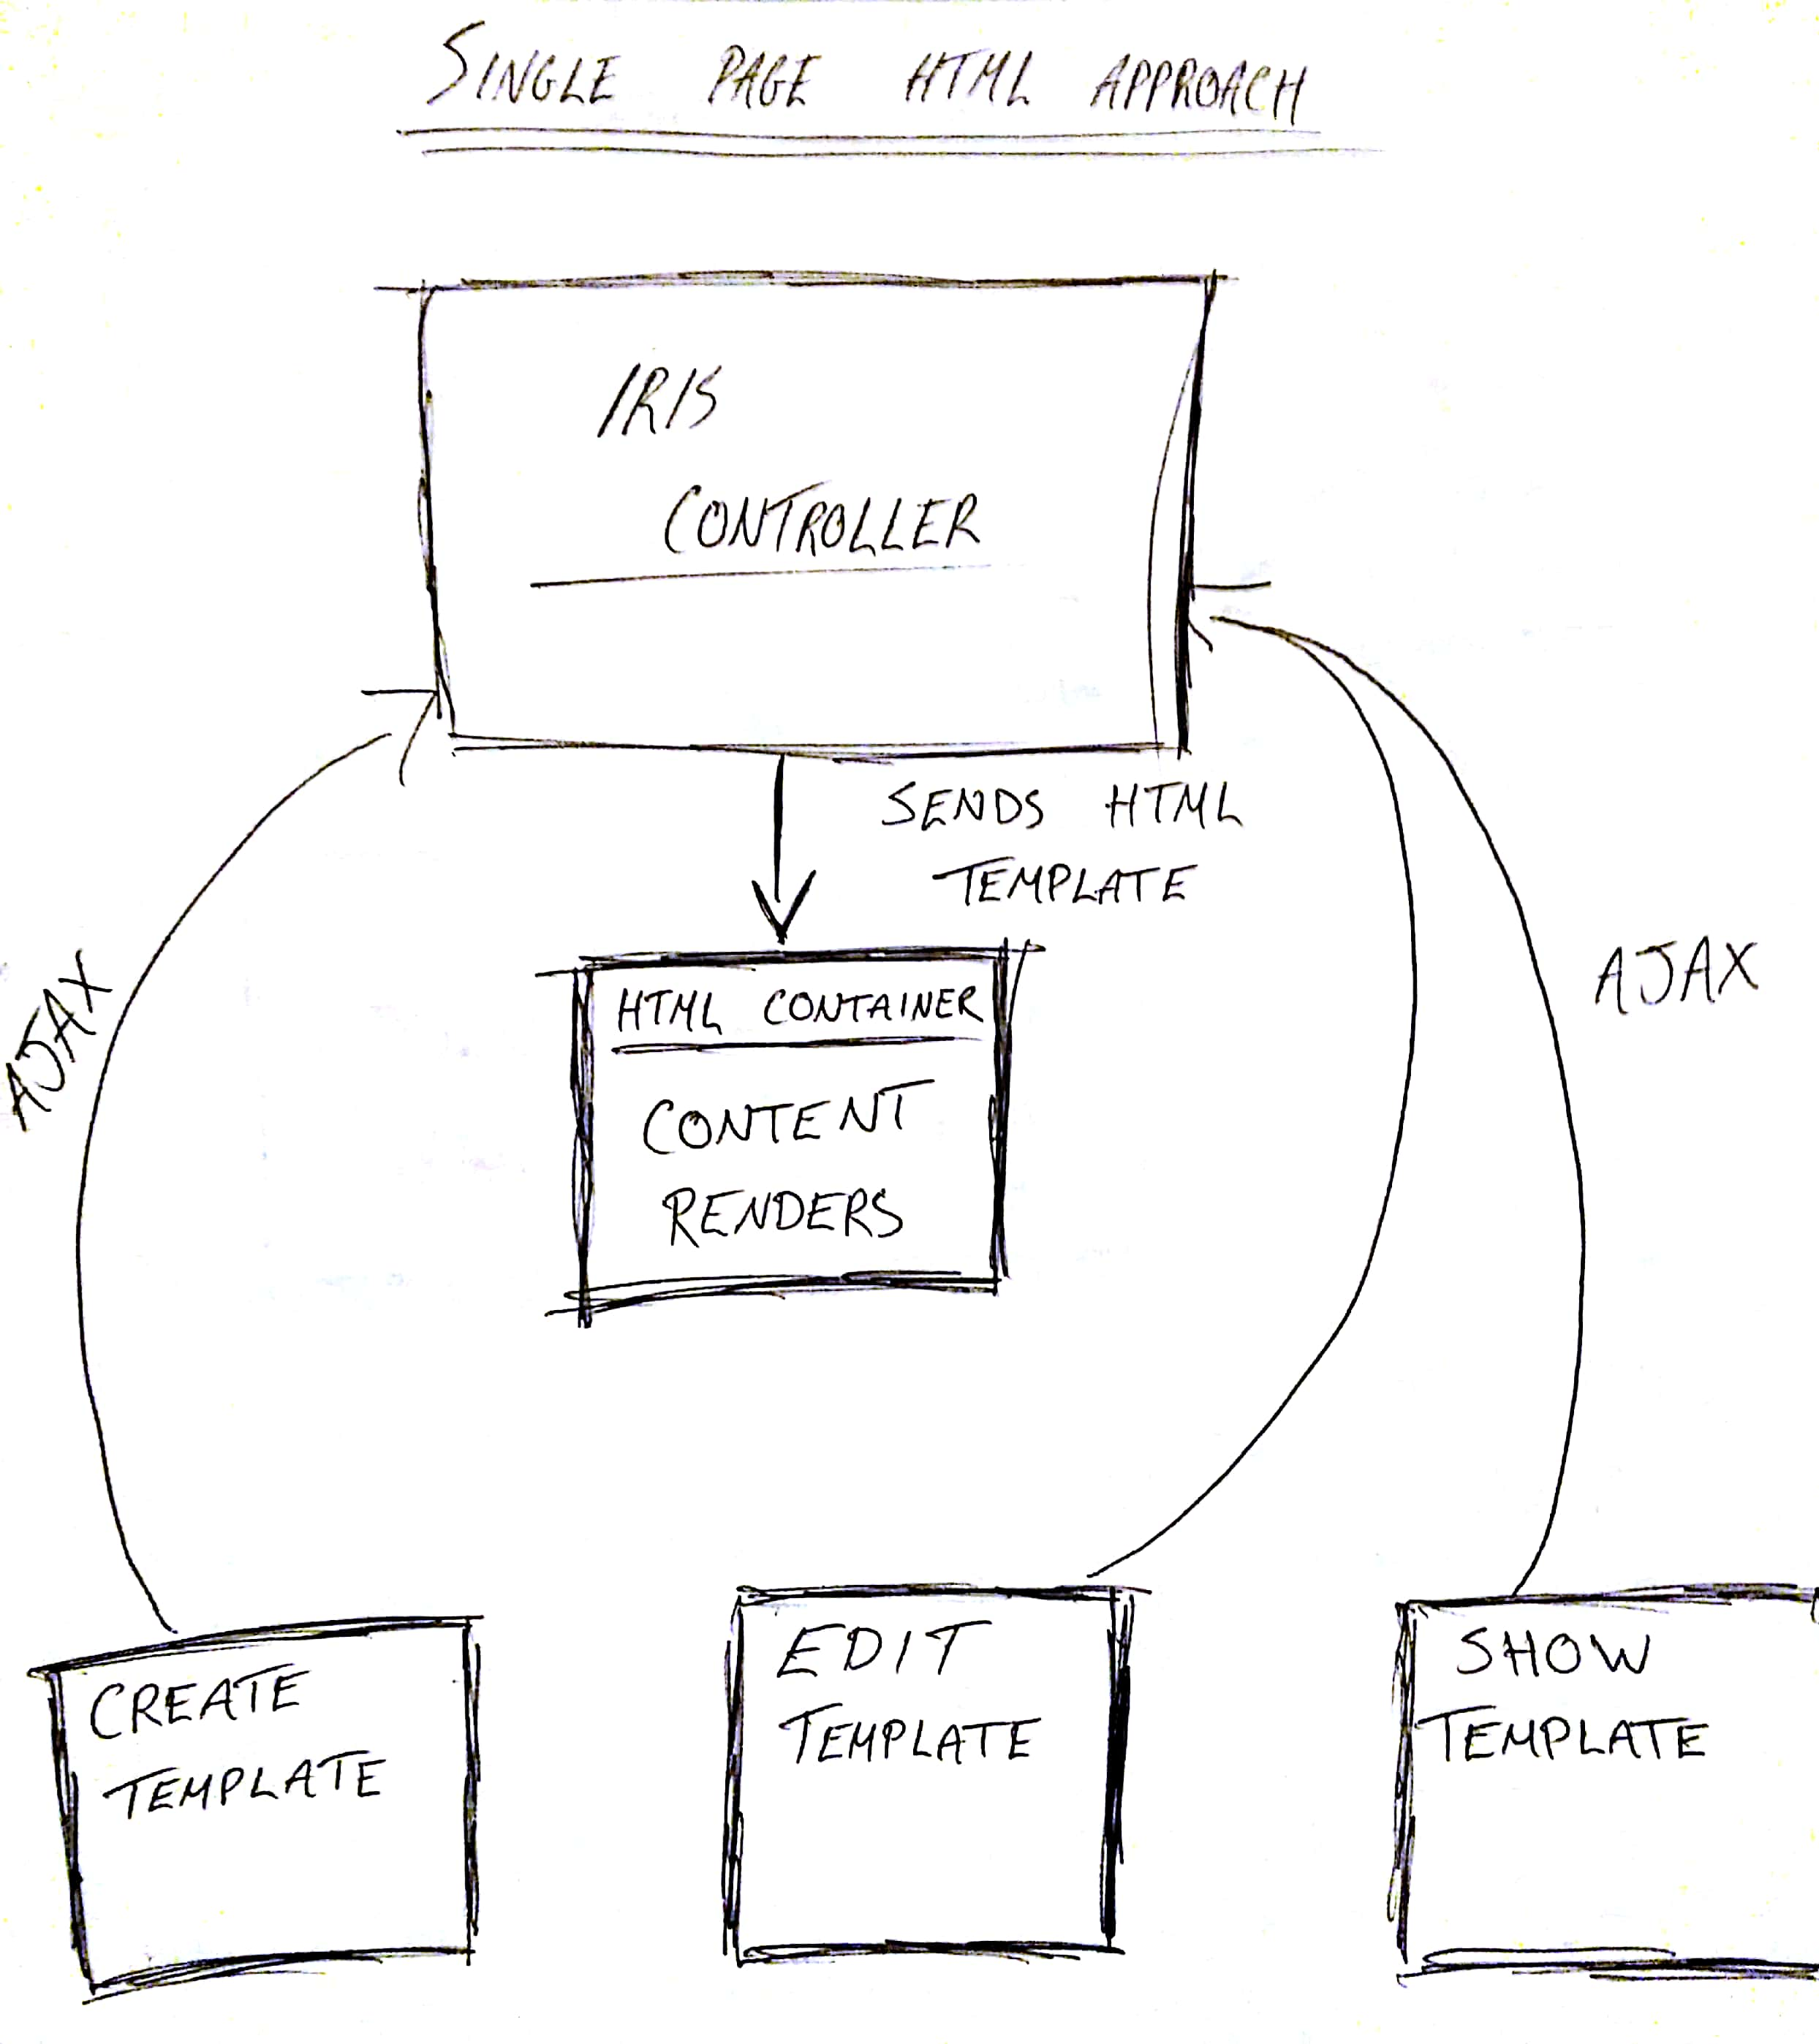
\includegraphics[width=\textwidth,height=\textheight,keepaspectratio]{single_html_container}
Iris will act as several single page web applications. As show in the diagram, each page will contain a main area for html content, which will be replaced by templates using ajax calls to the backend.
\end{tcolorbox}
\caption{Several Single Page Applications Design}
\end{figure}

\nocite{*}
\printbibliography

\pagebreak

\begin{appendices}
\chapter{Iris Iterations}\label{sec:iterations}

Currently Iris has had four different design iterations. The Iris’ current iteration was previously discussed, below are the other three designs that were considered for Iris in the early stages of development.

\section{ MEAN (MongoDB, Express, Angular, Nodejs) Stack}

Before any development had started on Iris there was talks of potentially implementing Iris using the MEAN stack. Due to Nodejs being one of the leading web frameworks it would have been unwise to not at least consider what an implementation may look like using the MEAN stack. However when Iris was planned out with Onaware, they did not want to develop Iris in Nodejs due to existing applications being built using Grails. The solution would not have differed dramatically as both Grails and Nodejs share similar concepts, meaning architecture would have been the only major difference. Below is a design showing class relationships to suit MongoDB.

\begin{figure}[H]
\begin{tcolorbox}
\centerline{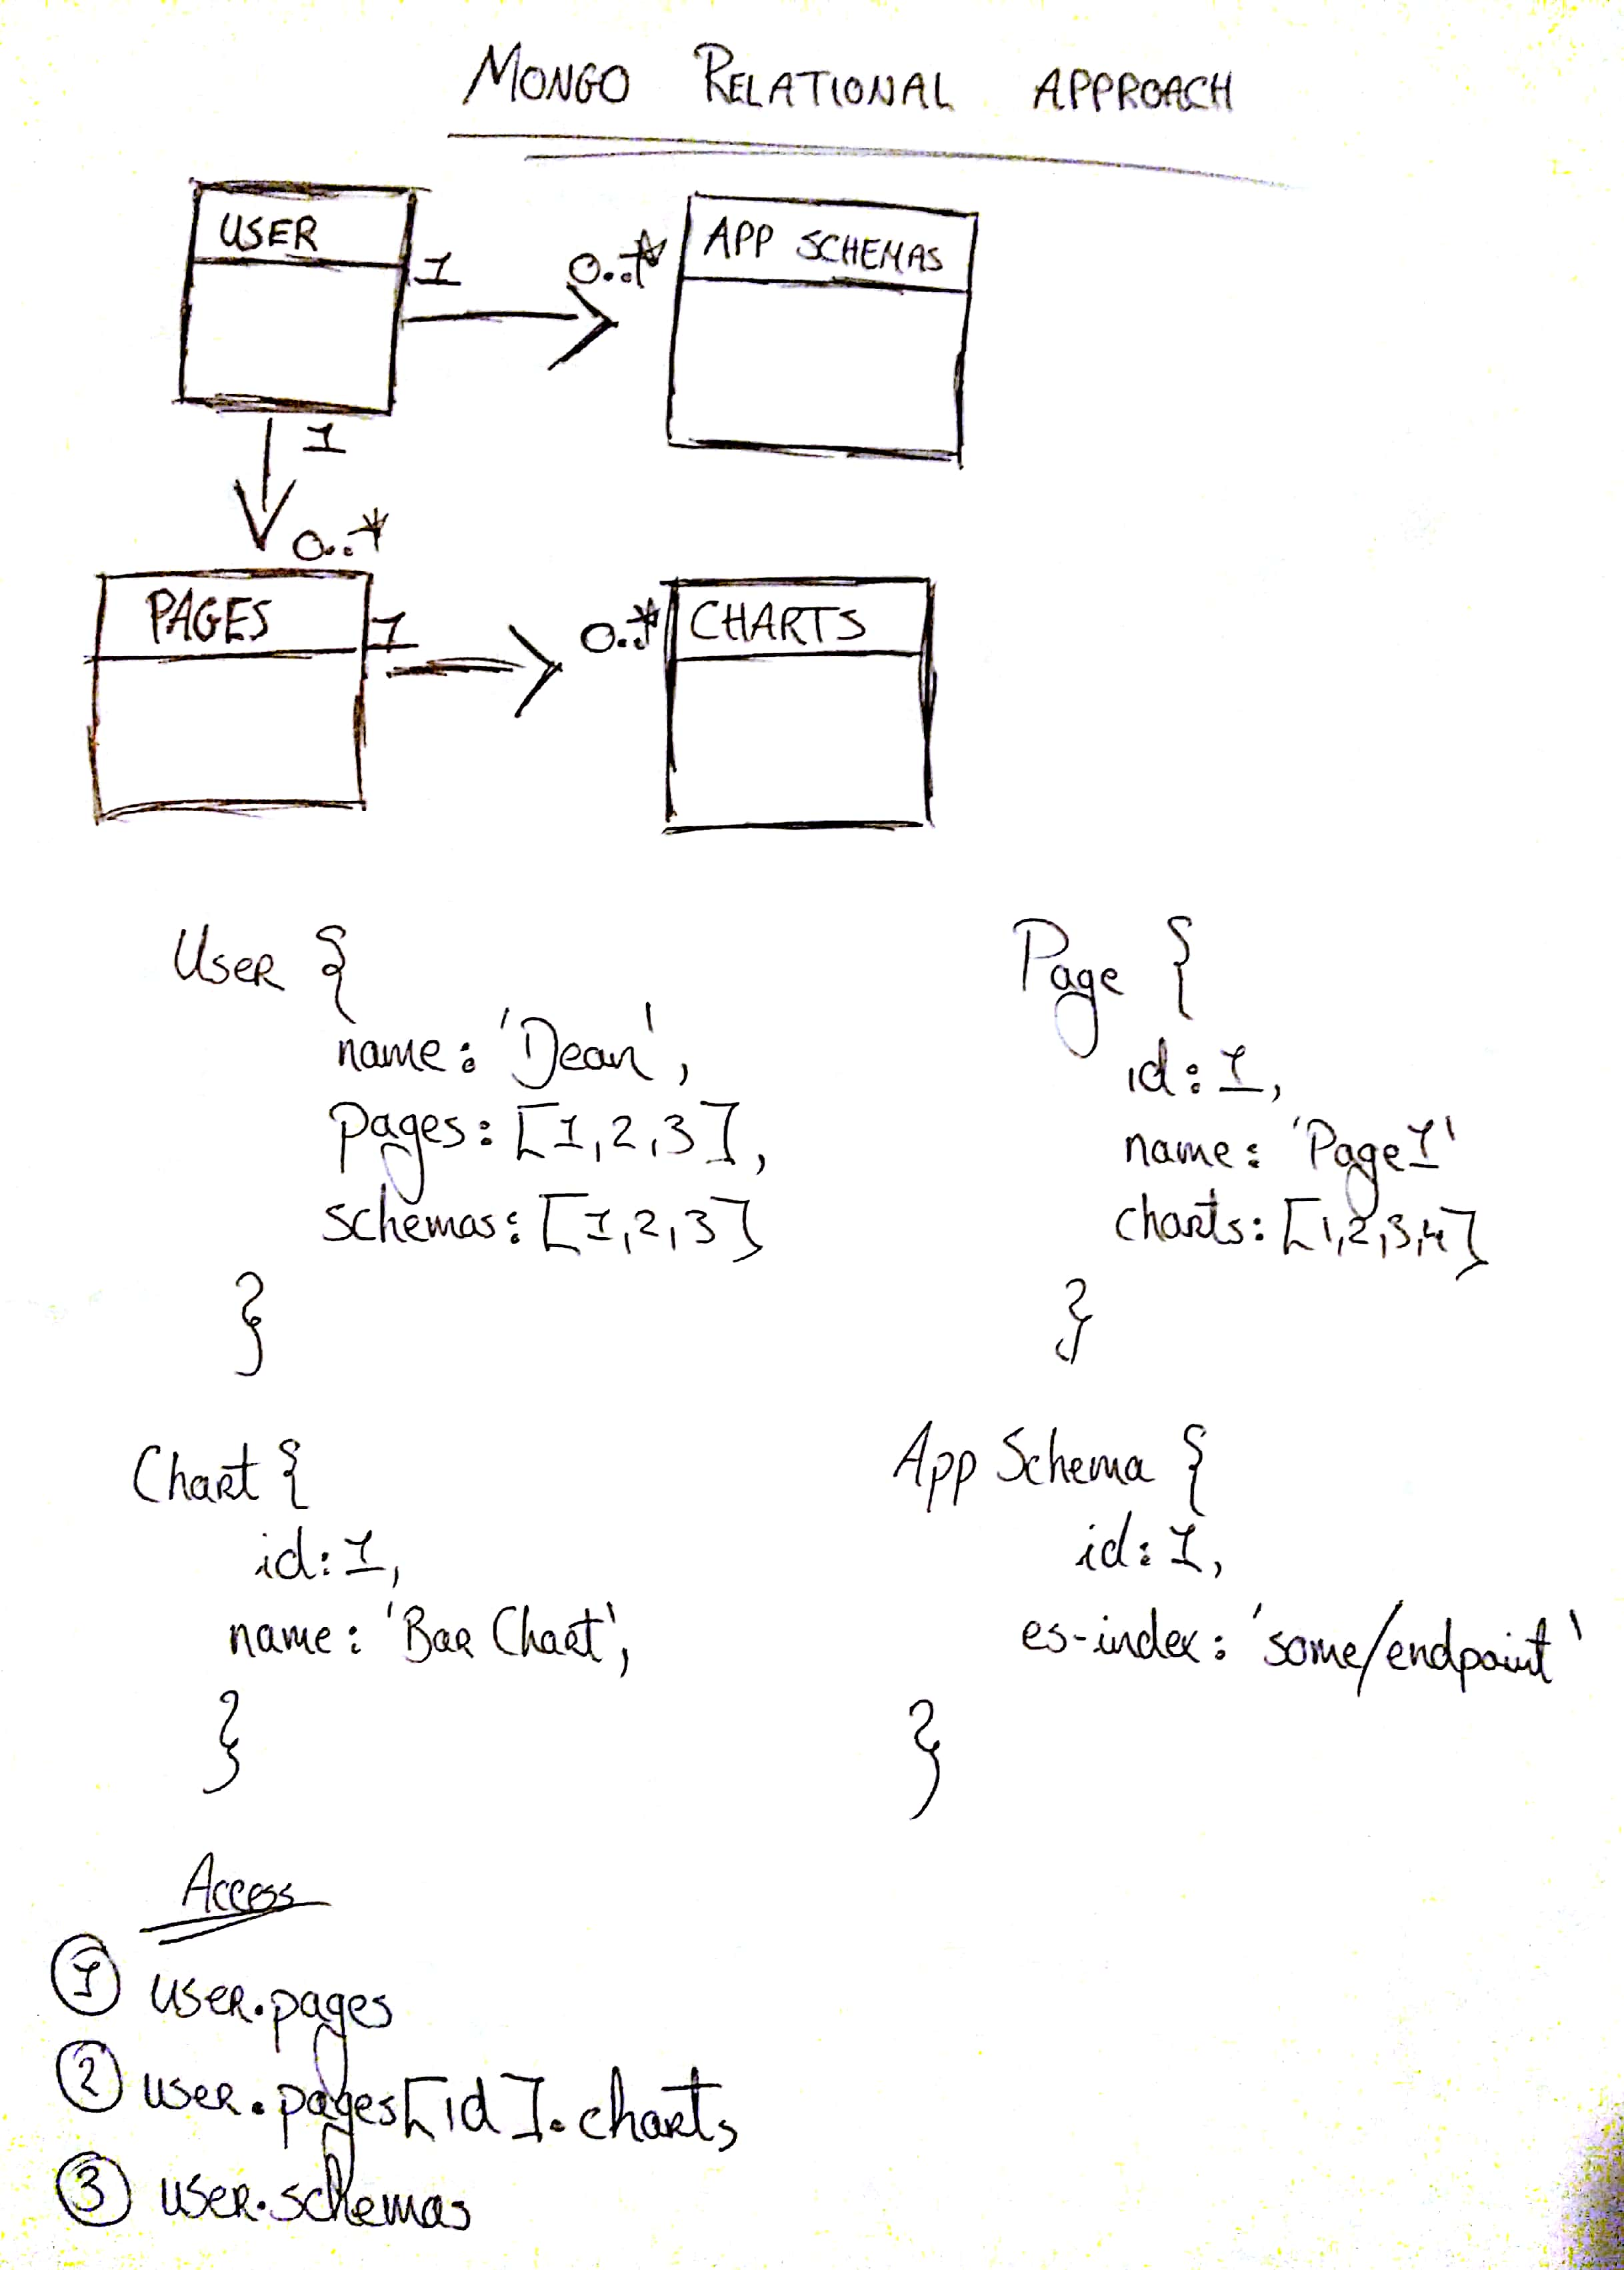
\includegraphics[width=\textwidth]{mongo_relation}}
How Iris may have looked using a relational approach to suit MongoDB.
\end{tcolorbox}
\caption{MEAN Stack Implementation}
\end{figure}

\section{Iris Single Page Application}

In the early stages of trying to understand how Iris would work, a single page application diagram was used to try and scale the design down to help as an understanding aid for those who did not understand the concept. Upon reviewing the diagram the implementation looked like a reasonable option. 

This implementation would have Iris a single entity where a user could use the web application as a means of pointing at a data source such as Elasticsearch and running analytics on the fly rather than having dashboards. The app would consist of one analytics page where a user picks their Elasticsearch endpoint and runs aggregations against it using a user friendly interface to build the aggregations. These aggregations could then be displayed on charts.

The issue with this idea is that it was very similar to Kibana and Grafana and only allowed a user to view their analytics but didn’t offer anything more to the user. The user would also have to set up their charts every time they wanted to use the application, this might be ok for on the fly analytics but when a user wants to monitor an application it should be a dashboard containing continuously updated. It is for this reason this design was dropped. 

\begin{figure}[H]
\begin{tcolorbox}
\centerline{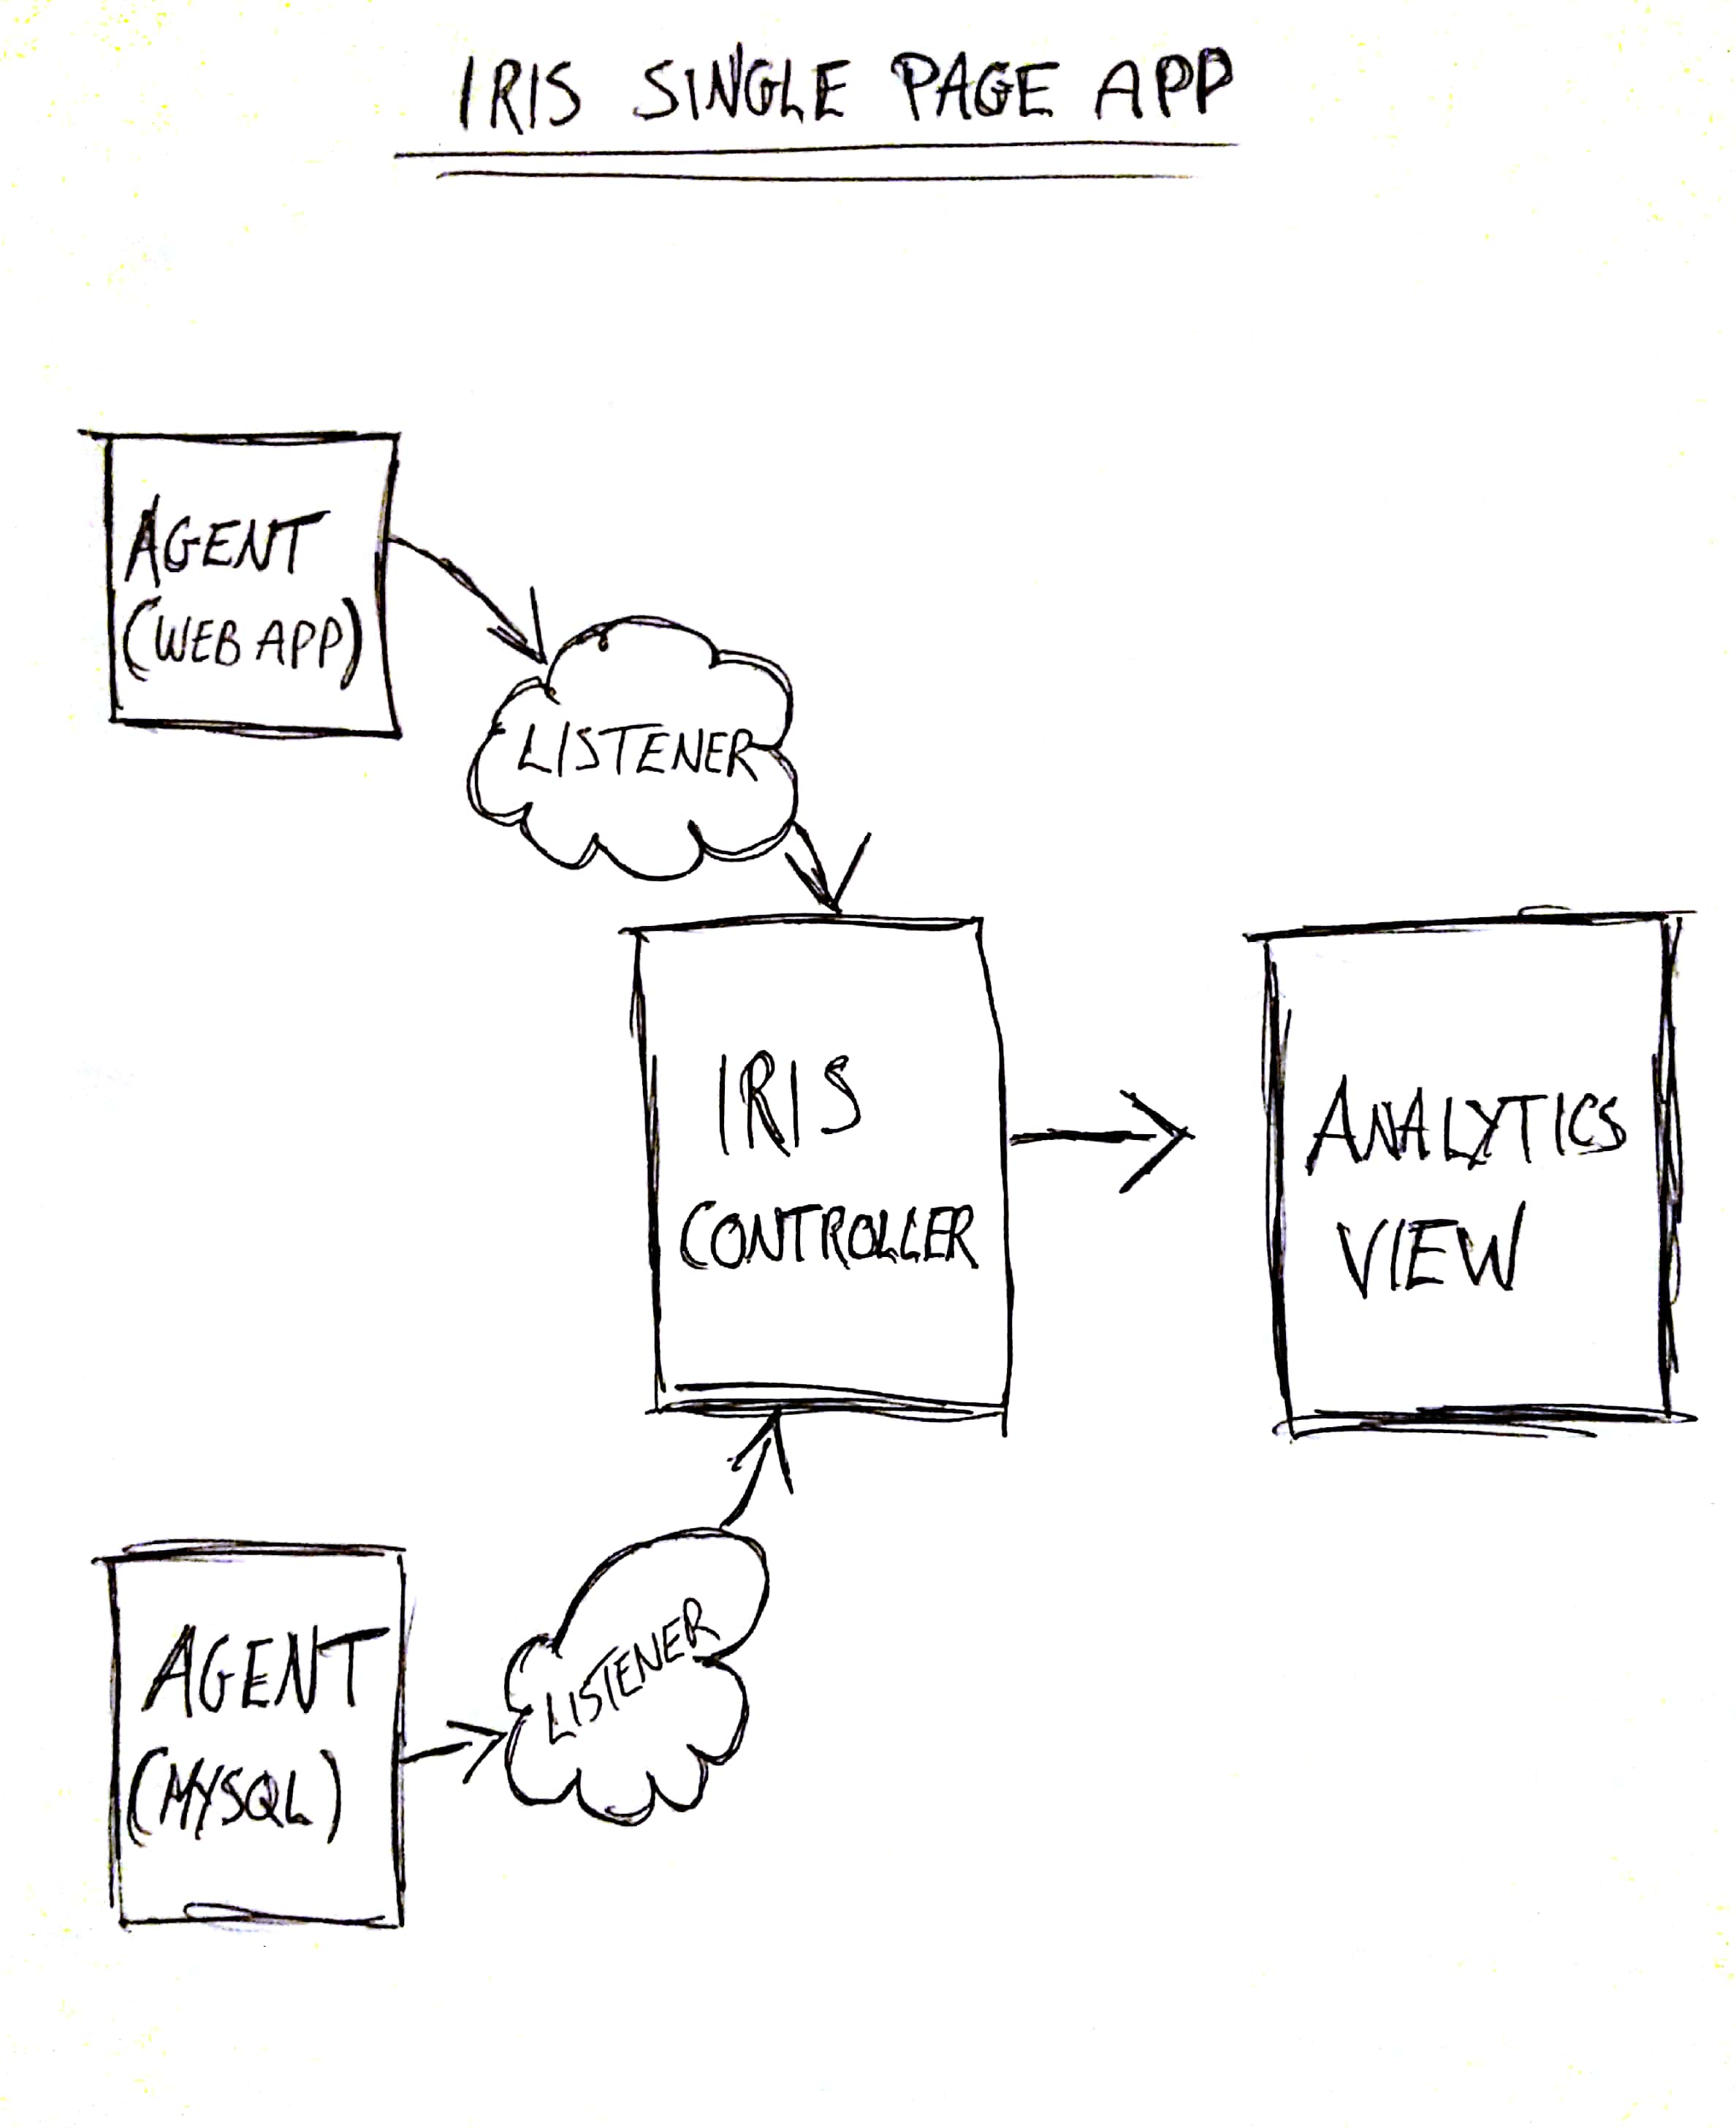
\includegraphics[width=.55\textwidth]{iris_single_page_app}}

Two applications are sending data to a single Iris controller action. A user then views this data using the single analytics view. This is how Iris might have looked as a single page application.
\end{tcolorbox}
\caption{Iris Single Page Application Implementation}
\end{figure}

\section{Iris \& Kibana as a Single Entity}

While researching similar products to Iris, Kibana was looked at extensively. During the research it was noted that Kibana is open source, meaning it may be possible to extend it rather than to build software to compete with it. Due to Kibana not allowing transformation of data and not allowing a user friendly way to insert data into Elasticsearch, Iris had advantages over Kibana. 

Rather than completely rebuild a dashboard system and an aggregation system, it is possible to use Kibana as a frontend for viewing your analytics and to use Iris as a means of routing, transforming and managing your data. This implementation would require a reverse proxy to be put in place to make Iris and Kibana appear as a single entity. The reverse proxy would redirect requests from Iris to Kibana and vice versa, making the two appear as a single entity.

This approach looks very appealing, as it would save a lot of work in having to make a dashboard system and an aggregation system. However because Kibana is public and has no concept of a user, the illusion of a single entity is broken when a user must sign into Iris and then doesn’t have to sign into Kibana. Another issue is when a user wants to go from Kibana back to Iris, Kibana must be modified to include links that redirect back to Iris this is doable seeing as Kibana supports plugins and is open source. However due to Kibana not supporting users; personal dashboards are no longer supported in the system which is something Iris wishes to achieve.

This kind of architecture is best suited for SSO (Single Sign On) technology such as Gluu. However the amount of  time required to implement a SSO solution along with building a piece of software to integrate with existing software scales the project and it becomes difficult to estimate a completion time. It is for this reason and the lack of personalised aspects of Kibana that Iris will be a standalone application.

\begin{figure}[H]
\begin{tcolorbox}
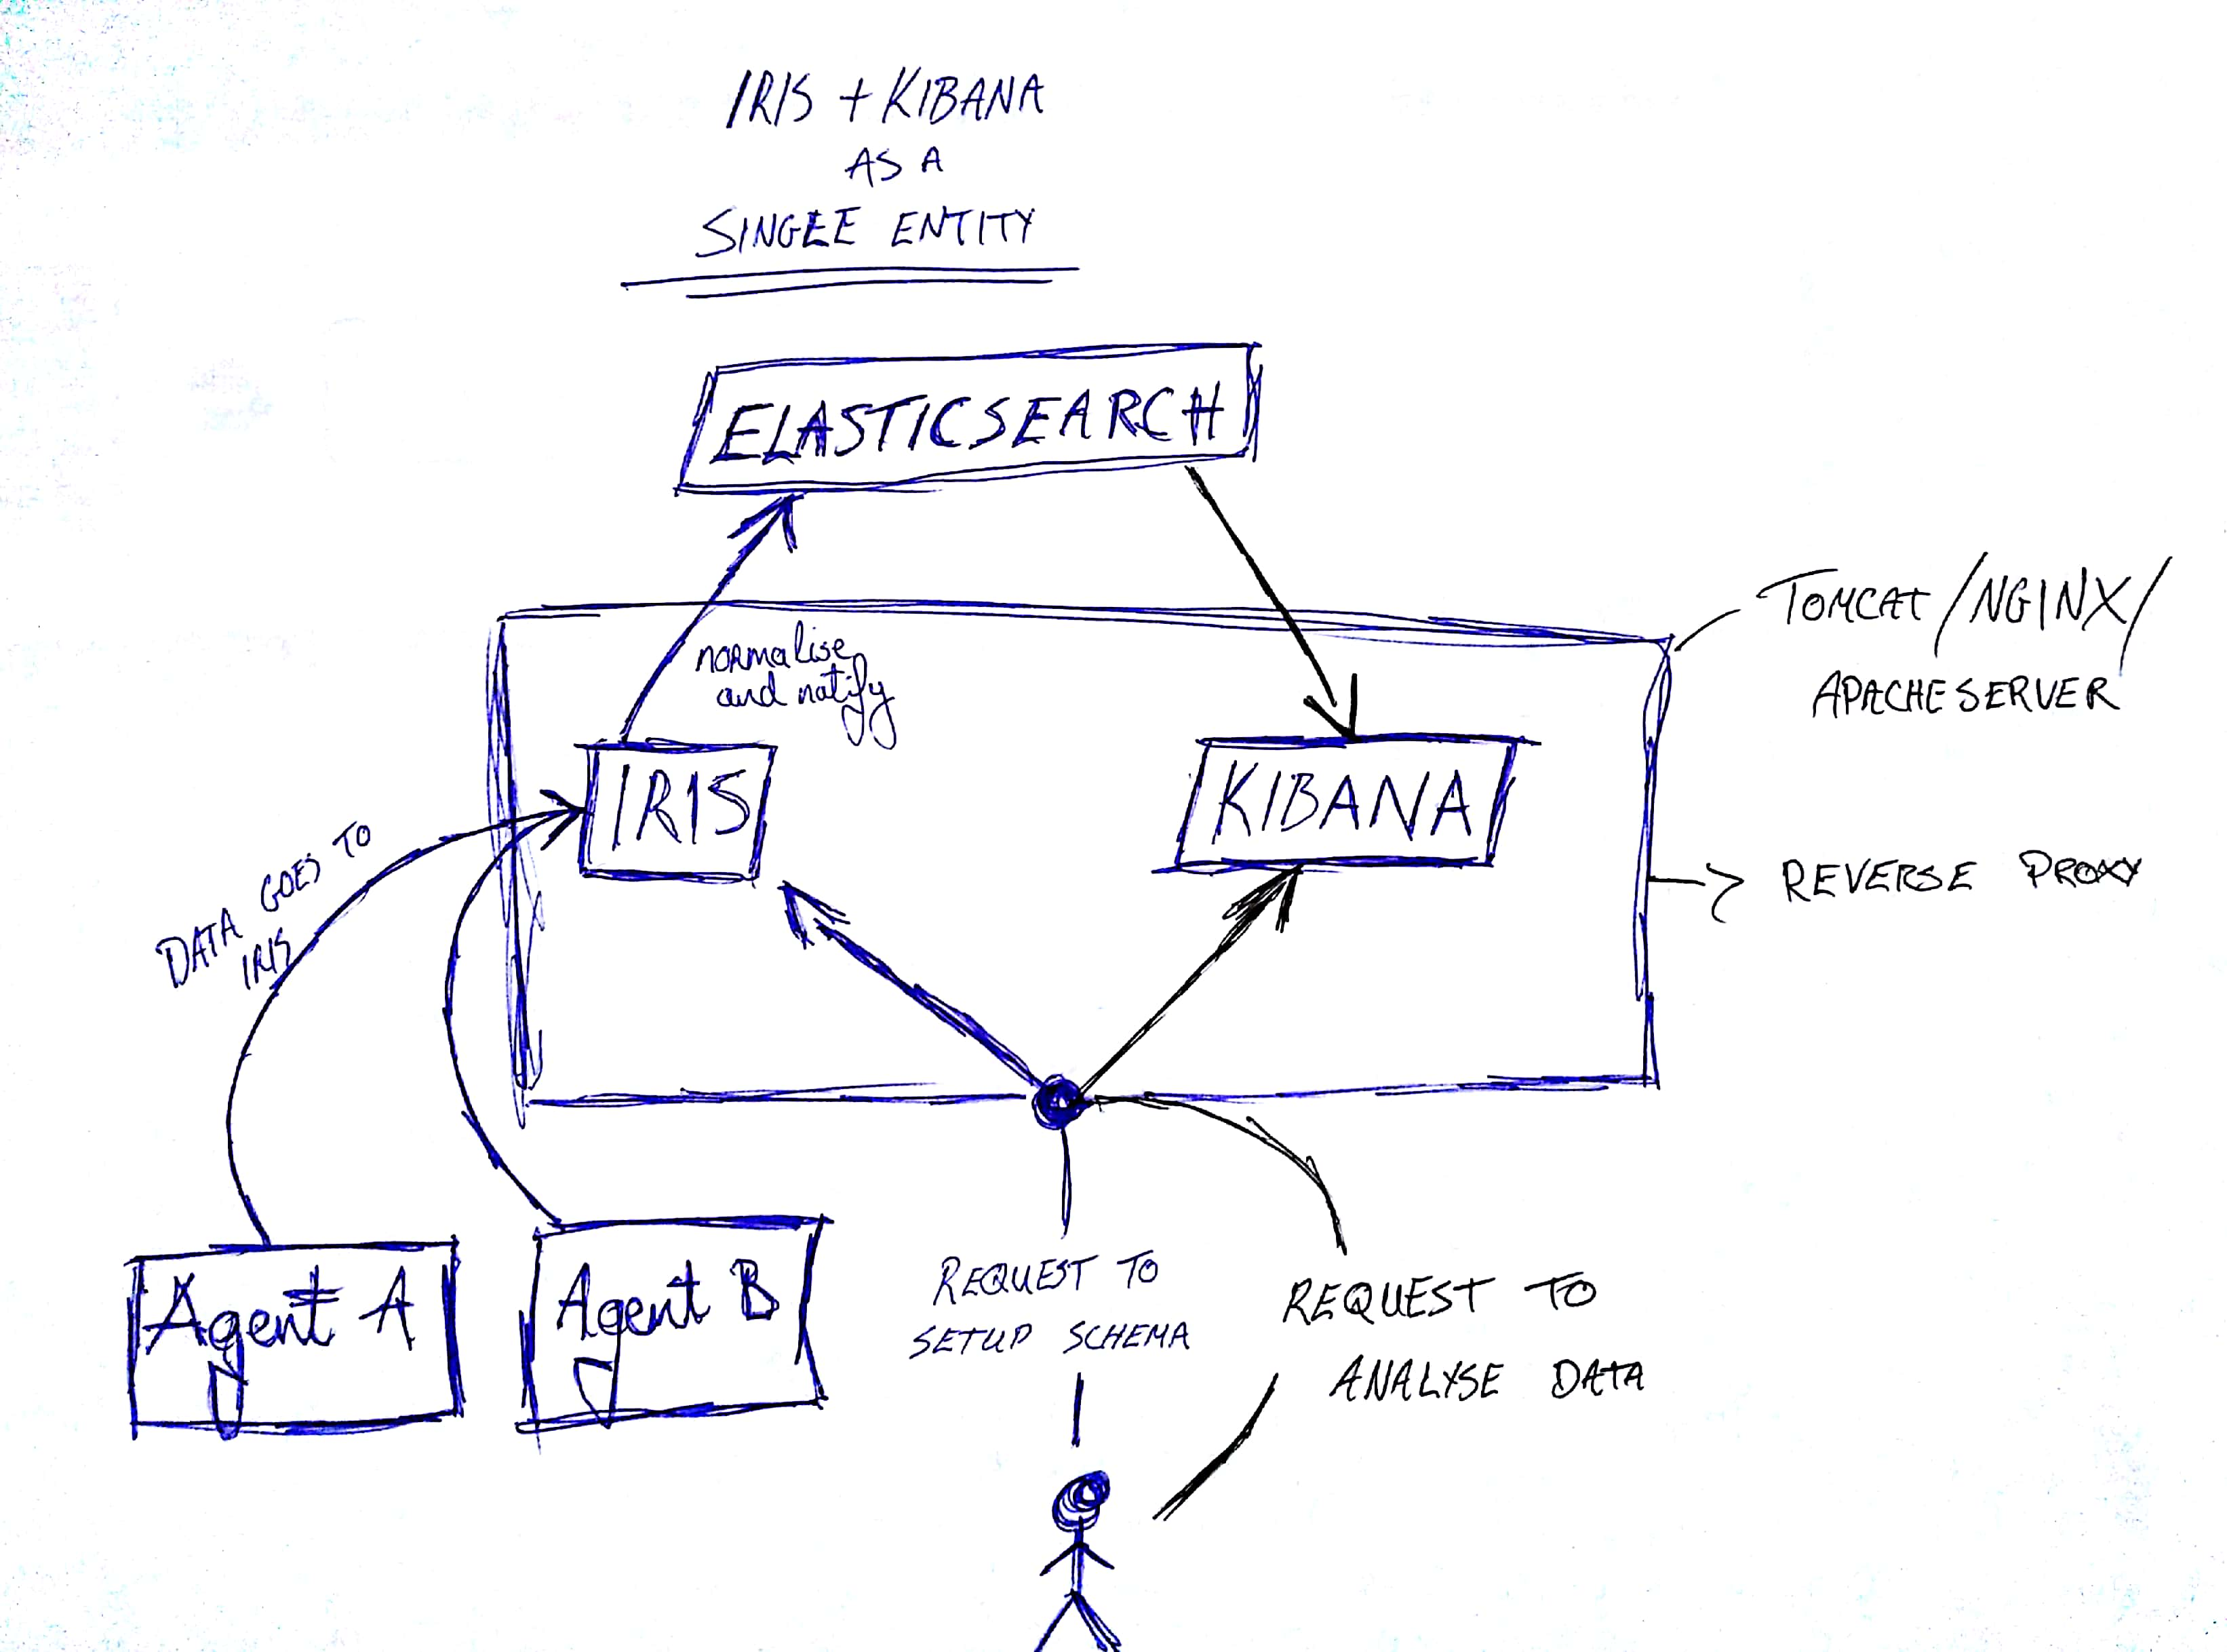
\includegraphics[width=\textwidth,height=\textheight,keepaspectratio]{iris_kibana_single_entity}
\newline
Iris and Kibana working together as a single entity.
\end{tcolorbox}
\caption{Iris \& Kibana as a Single Entity}
\end{figure}
Documentation on Gluu can be found here \url{https://gluu.org/docs/}

\chapter{Iris Trello Board}\label{sec:trello}

Iris’ issues and sprints are being tracked using Trello. These are organised using the kanban system and custom labels inside of Trello. Trello allows filtering of cards by their labels, meaning issues related to a particular sprint can be the only cards visible. This makes tracking sprints and issues for the sprint easy to manage.

\begin{figure}[H]\centering
\begin{tcolorbox}[text width=.8\textwidth]
\centerline{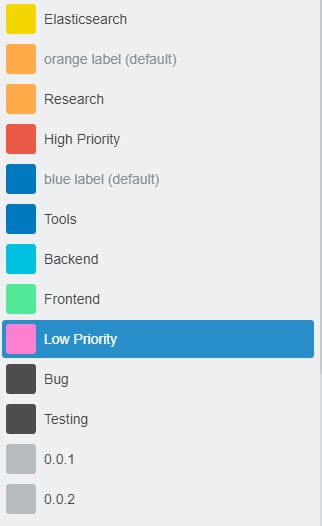
\includegraphics[width=.4\textwidth]{trello_labels}}

Here are some of the labels being used to manage Iris issues in Trello.
\end{tcolorbox}
\caption{Iris’ Trello Labels}
\end{figure}

\begin{figure}[H]
\begin{tcolorbox}
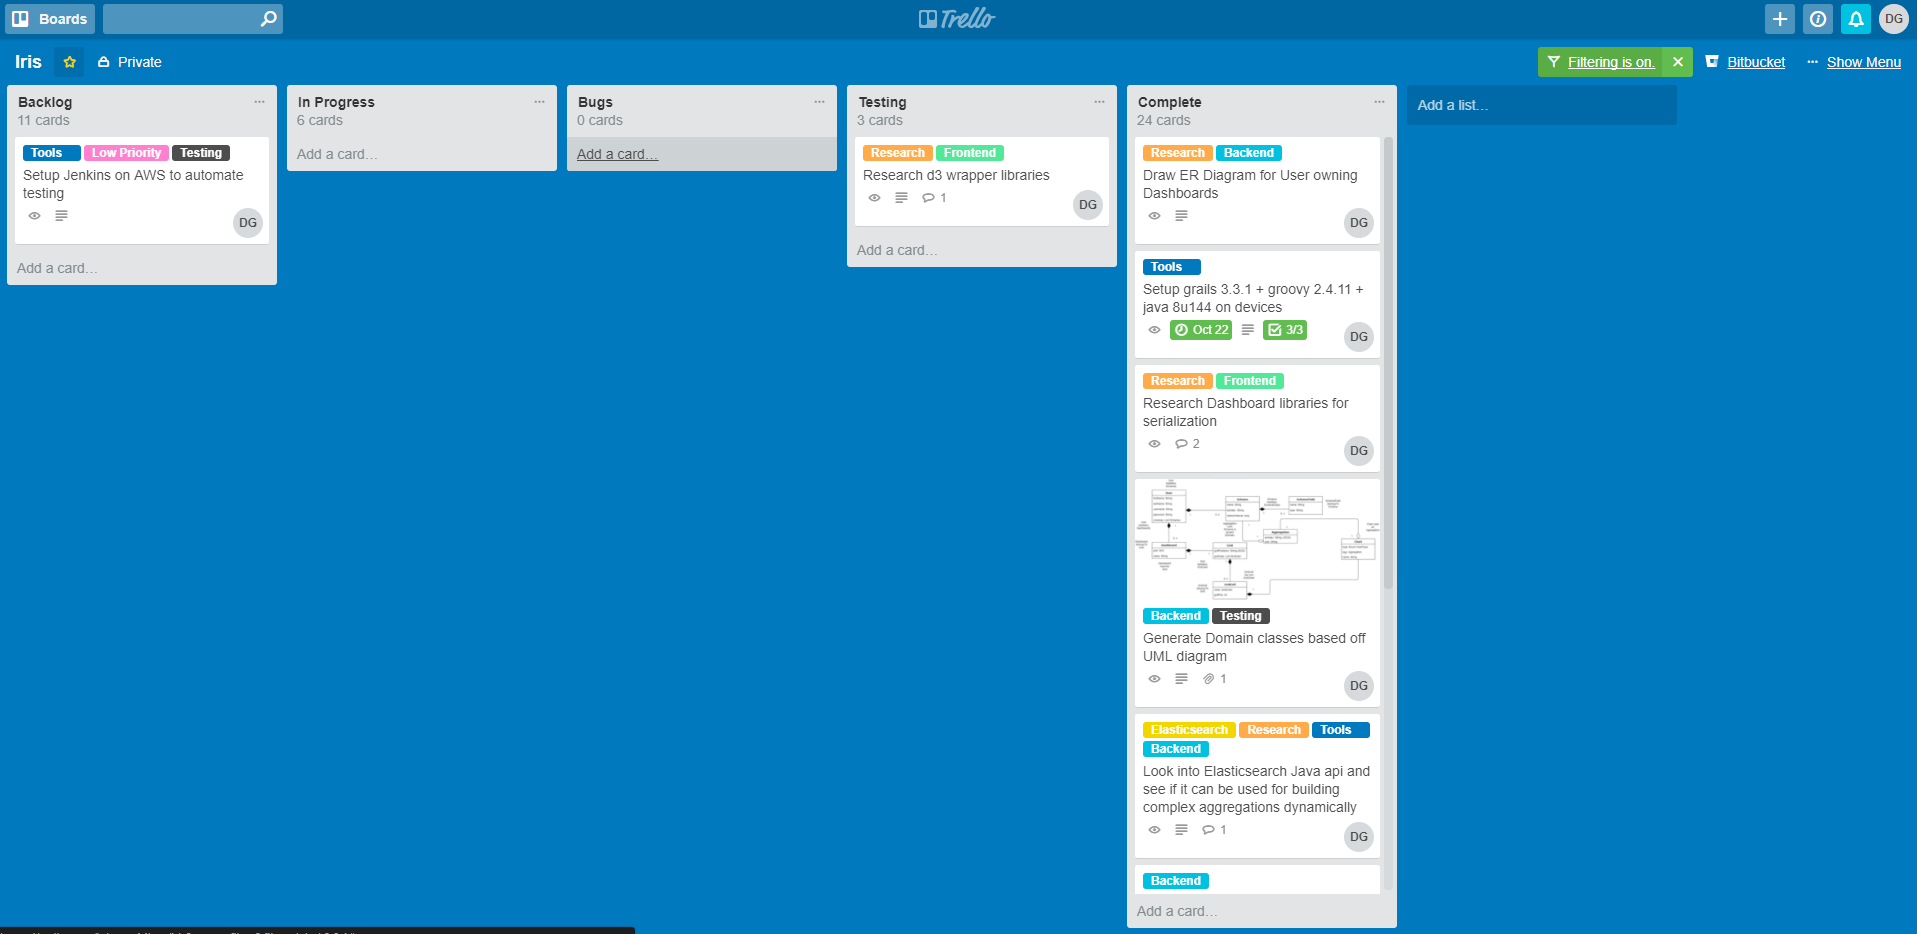
\includegraphics[width=\textwidth]{trello_sprint_1}
\newline
An image of the Trello issues for the first sprint of Iris, containing label 0.0.1
\newline
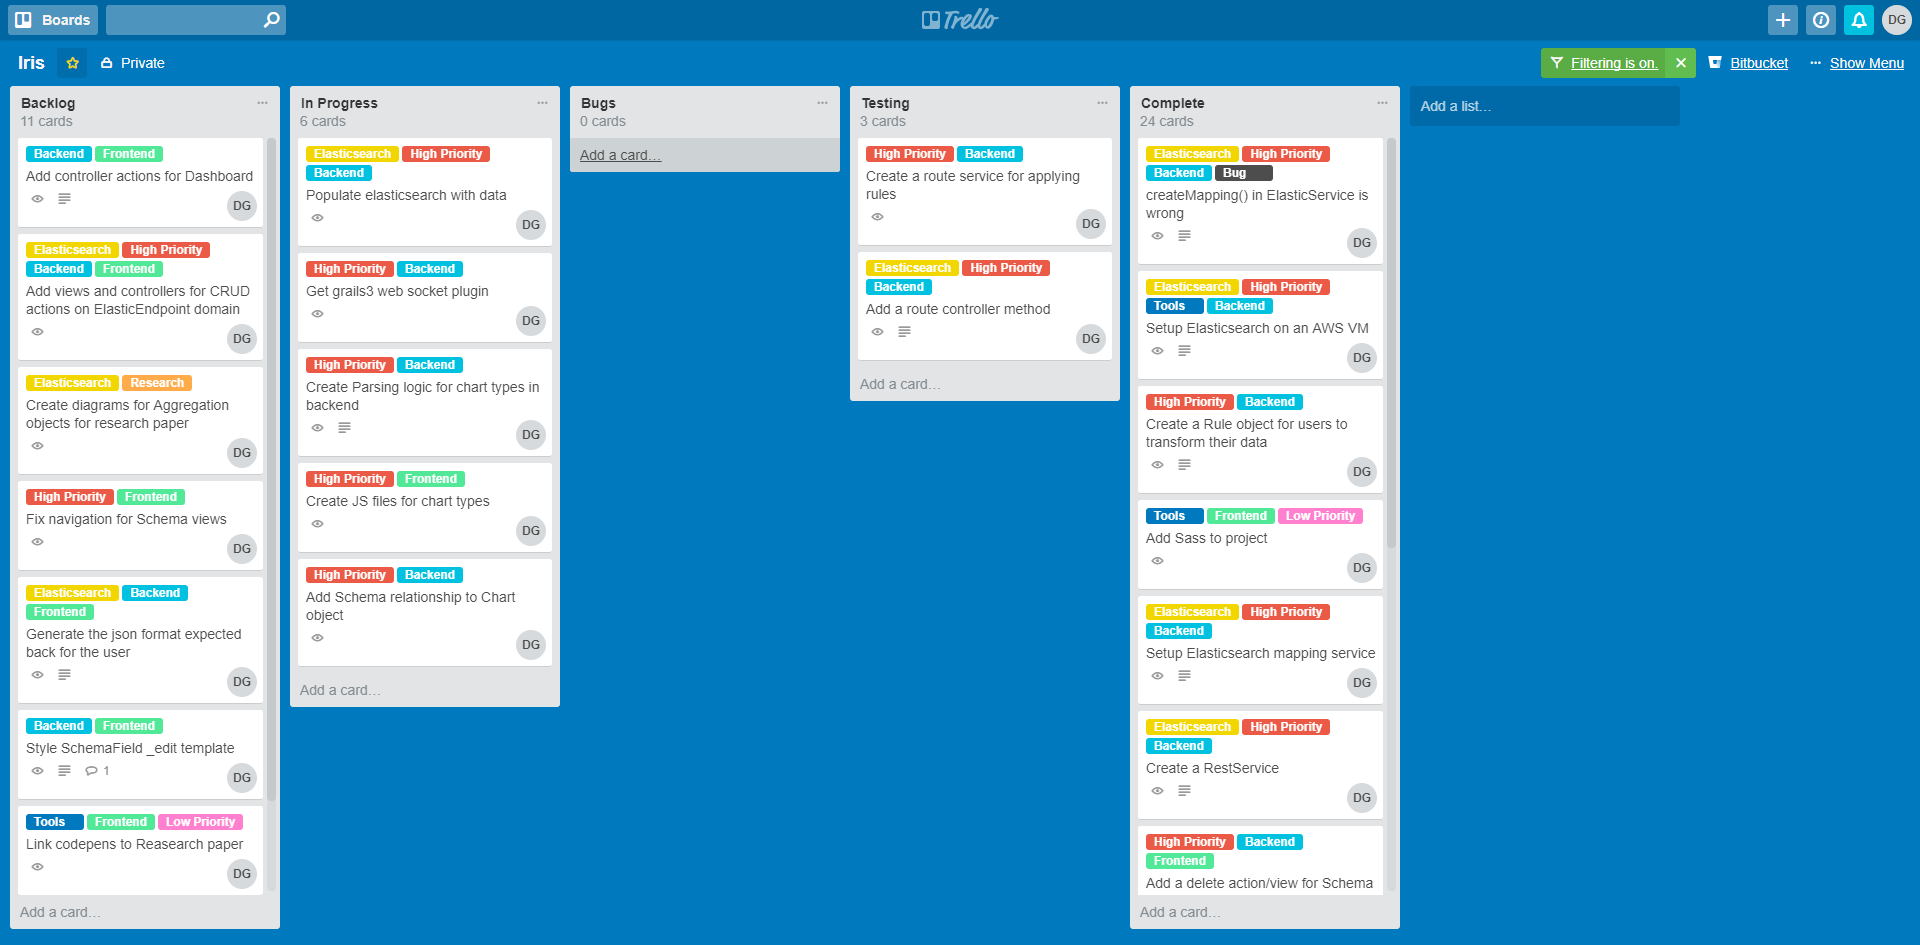
\includegraphics[width=\textwidth]{trello_sprint_2}
\newline
An image of the Trello issues for the second sprint of Iris, containing label 0.0.2
\end{tcolorbox}
\caption{Iris Sprint Issues}
\end{figure}

\chapter{Dashboard Library Comparisons}\label{sec:dashboards}

Some time was spent researching dashboard libraries that could be used in Iris, below are the four libraries compared in detail.

\section{Gridster}

Gridster (\url{http://dsmorse.github.io/gridster.js}) is a great candidate for controlling the dashboard functionality in Iris as it covers all of the requirements needed. The biggest advantage of using Gridster for Iris is that the dashboard can be serialized as a JSON object which is perfect for saving and restoring dashboards. The only issue with Gridster is that it is no longer in active development which means if any issues occur it becomes extremely difficult to get support for the issue being tackled.

Gridster demos can be found here \url{http://dsmorse.github.io/gridster.js/#demo}

\section{Packery}

Packery (\url{https://packery.metafizzy.co}) is arguably one of the most popular grid libraries. However Packery is not suited for Iris as it is doesn’t come with serialisation built into the library. Serialisation can be achieved but it requires a lot of understanding of the library to see how it can be implemented. The main reason Iris can not use Packery is due to it not being under the MIT license — a requirement for Onaware.

\section{GridList}

GridList (\url{https://github.com/hootsuite/grid}) is a library which takes a different approach to grid systems compared to Gridster. Upon reading GridList’s API it seems to have a very small amount of functionality open to the developer. There was no sign of common functions to add or remove widgets, it looked like DOM elements needed to already be in place before they could be turned into Grid items, which is not ideal for Iris as Iris needs to be able to add grid items dynamically. It is for this reason Iris will not be using GridList to implement a dashboard system.

\section{GridStack}

GridStack (\url{http://gridstackjs.com/}) is an expanded version of Gridster, it carries the same functionality as Gridster as well as some extra functionality. A major reason for GridStack being useful for Iris is that the developer is very active on github and is quick to reply to issues. The developer also spends time helping people adapt Gridstack to people's specific needs which is perfect for something like Iris as it is hard to tell in the early stages of development what issues may arise in the later stages of the project. Gridstack also meets all of the requirements needed for Iris.

Gridstack demos can be found here \url{http://gridstackjs.com/demo/}



\chapter{Chart Library Comparisons}\label{sec:charts}

Some time was spent researching chart libraries that could be used in Iris, below are the four libraries compared in detail.

\section{Why D3 is not being used directly}

D3 is one of the most popular visualization libraries at present. The library allows a great amount of control over your data visualization and has a very powerful API. The issue with D3 is that it has a steep learning curve and would require a lot of time to understand how the charts are being constructed. D3 is also very raw by nature as it is essentially a visualization library not a chart library and requires you to implement your own legends and axis. This puts a lot more work on the developer. Due to the large scale of Iris a library which comes with these features is preferable. D3 has recently moved up to v4, the majority of tutorials and examples available for D3 are implemented in v3, due to v4 being relatively new. This means Iris would either have to use a the older version of D3 to ensure stability or attempt to implement the charts in the newer version which has less resources to learn from.

\section{C3}

C3 (\url{http://c3js.org/gettingstarted.html}) is a wrapper library for D3v3, the library focuses on taking away the boilerplate code needed to implement charts in plain D3. C3 manages to achieve this by providing axis, legends, chart constructors and easy data manipulation immediately without any extra code. C3 suits all of the charting requirements for Iris which makes it a promising candidate. The issue with C3 is that it is based on D3v3. Due to C3 being based on the older version of C3, it seems that development has slowed down on C3 and there isn’t active support on their Github. Iris would benefit more as a new system by working with newer versions of libraries.

C3 demos can be found here along with the code for creating the charts \url{http://c3js.org/examples.html}


\section{Billboardjs}

Billboardjs (\url{https://naver.github.io/billboard.js}) is a wrapper library for D3v4, it is also a fork from C3. Billboard was created to solve the issues mentioned previously, which was to port the functionality of C3 to a new library which supported D3v4. Due to Billboardjs being a fork of C3, they carry the same functionality which is ideal for Iris. Billboardjs has an excellent API and their documentation is very well laid out. 

Based on the research to date Billboardjs does not appear to have any issues which will affect Iris, so is currently the most likely charting component for use with Iris.

Billboardjs examples can be found here along with the code for creating the charts \url{https://naver.github.io/billboard.js/demo/}

\section{Chartjs}

Chartjs (\url{http://www.chartjs.org/docs/latest/getting-started/}) is a popular lightweight charting library which aims to simplify chart construction by automatically supporting legends, axis, zooming, panning and responsiveness. Chartjs has a very active community and has been compared to D3 without the complexity. Chartjs has a limited amount of charts to choose from, but users of the library are actively creating add ons supporting additional charts. 

Due to Iris having another lifecycle after this project cycle it is preferable to select a larger charting library with more features in order to satisfy, as yet, unfinalised  requirements.

Chartjs demos can be found here \url{http://www.chartjs.org/docs/latest/charts}
\end{appendices}
\end{document}